\chapter{零阶随机优化}
\label{chap:zeroth-order-optimization}

设想调节一台仿真器的两个参数。把参数填进去，运行一次，仿真器吐出一个代价数字。它的内部是几十万行别人写的程序，没有人能告诉你代价对参数的导数，甚至不确定这个导数处处存在。此前各章每一步都要读梯度，这里没有梯度可读，能做的只是换一组参数再试一次。

这样的处境里，局部方向只能靠函数值的差别来构造。\term{零阶优化}（zeroth-order optimization）指只使用函数值的优化，“零阶”相对于用梯度的一阶和用Hessian的二阶而言。本章讨论其中用随机扰动构造方向的一类方法，称为\term{零阶随机优化}（zeroth-order stochastic optimization，ZOSO）。全章用同一个目标核对每一步：
\begin{equation}
 f(\bm{x})=\frac12\bigl(x_1^2+9x_2^2\bigr),\qquad
 \bm{x}^{(0)}=(9,1).
 \label{eq:zo-example}
\end{equation}
它的梯度是$\nabla f(\bm{x})=(x_1,9x_2)$，$L=9$，$\mu=1$，起点处$f=45$，$\nabla f=(9,9)$。这些量只用来检查算法，算法本身看不到表达式，只能读数。

第~\ref{sec:zo-feedback}节先说清一次查询返回什么，因为后面所有结论都依赖这个接口。第~\ref{sec:zo-finite-differences}节用差商逼近原目标的梯度，会遇到两个对手：扰动尺度太大时的截断误差，太小时被放大的读数噪声。第~\ref{sec:zo-smoothing}节换一种看法：不去逼近原梯度，而是把目标在邻域上平均一下，于是函数值能够给出这个平均目标梯度的无偏估计。

有了方向，第~\ref{sec:zo-method}节把它接进迭代，需要分清算法到底在优化哪个目标。第~\ref{sec:zo-error-cost}节按函数读数次数比较各种方法，并回答最后一个问题：在平滑目标上得到的结论，对原目标意味着什么。

\section{函数值反馈}
\label{sec:zo-feedback}

调节仿真器参数时，算法与仿真器之间到底交换什么信息？同样叫“只能读函数值”，读数是否带噪声、一轮能读几个位置、两次读数能否共用一次仿真，会让后面的误差结论相差几个量级。所以先把接口固定下来。

\paragraph{目标、查询点与读数}
我们要最小化$f(\bm{x})$，$\bm{x}\in\bm{C}\subseteq\mathbb{R}^n$。算法每次提交一个\term{查询点}（query point）$\bm{q}\in\mathbb{R}^n$，黑箱返回一个实数$y$，称为\term{读数}（reading）。查询点不一定等于当前迭代点，算法常常故意偏离当前点一点，再比较读数。

这里出现两种性质不同的随机性，如图~\ref{fig:zo-feedback}所示。第一种在算法内部：算法自己抽取偏离的方向，这是我们主动加入的。第二种在黑箱内部：同一个查询点运行两次，可能因为测量噪声或仿真种子不同而得到不同的读数，这是我们无法控制的。

\begin{BookInlineFigure}
  \centering
  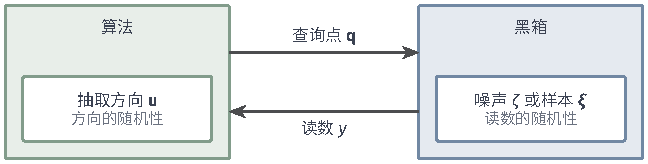
\includegraphics[width=110mm]{figures/05-optimization/05-stochastic-optimization/tikz/zo-feedback/figure.pdf}
  \caption{零阶优化的接口。算法提交查询点$\bm{q}$，黑箱返回读数$y$。方向$\bm{u}$的随机性由算法产生，噪声$\zeta$或样本$\bm{\xi}$的随机性来自黑箱，二者相互独立地起作用，分析时分别记录。}
  \label{fig:zo-feedback}
\end{BookInlineFigure}

\subsection{精确函数值与含噪读数}
\label{sec:zo-readings}

按黑箱内部的情况，读数分成三种模型。图~\ref{fig:zo-readings}画出了它们在一条一元曲线上的样子。

\paragraph{三种读数模型}
第一种是精确函数值，同一点读多少次都是同一个数：
\begin{equation}
 y=f(\bm{q}).
 \label{eq:zo-reading-exact}
\end{equation}
第二种是带\term{加性噪声}（additive noise）的读数，真实值上叠加一个随机误差$\zeta$：
\begin{equation}
 y=f(\bm{q})+\zeta.
 \label{eq:zo-reading-additive}
\end{equation}
第三种是期望目标的样本函数值。目标本身定义成随机函数的平均，一次读数对应一个随机场景$\bm{\xi}$：
\begin{equation}
 f(\bm{x})=\mathbb{E}_{\bm{\xi}}\bigl[F(\bm{x};\bm{\xi})\bigr],\qquad
 y=F(\bm{q};\bm{\xi}).
 \label{eq:zo-reading-sample}
\end{equation}

后两种的差别在于噪声是否依赖位置。贯穿例上取样本函数$F(\bm{x};\bm{\xi})=f(\bm{x})+\bm{\xi}^\top\bm{x}$，$\bm{\xi}$均值为零。场景$\bm{\xi}=(0.2,-0.1)$在起点给出
\[
 F(\bm{x}^{(0)};\bm{\xi})=45+0.2\cdot9-0.1\cdot1=46.7.
\]
这里偏差$1.7$随$\bm{x}$线性变化。固定一个场景，$F(\cdot;\bm{\xi})$是一条完整的曲线，如图~\ref{fig:zo-readings}(c)；而加性噪声模型里每次读数的误差是孤立的一个数，没有“这条曲线”可言。

\begin{BookInlineFigure}
  \centering
  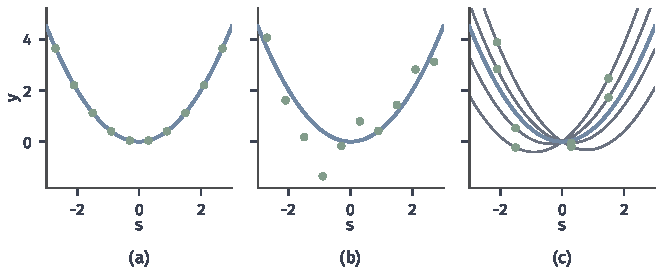
\includegraphics[width=112mm]{figures/05-optimization/05-stochastic-optimization/matplotlib/zo-readings/figure.pdf}
  \caption{同一个目标$s^2/2$（蓝线）的三种读数，绿点是读数。(a)精确读数落在曲线上。(b)加性噪声读数在曲线上下散开，标准差$0.6$。(c)样本函数$s^2/2+\xi s$，取四个场景$\xi$（灰线），绿点是同一场景曲线上的读数，蓝线是它们的期望。}
  \label{fig:zo-readings}
\end{BookInlineFigure}

\paragraph{无偏须对给定的历史和查询点成立}
什么叫“读数没有系统偏差”？直观要求是平均起来等于真值。但这个平均必须在“算法已经知道的一切”都固定时计算，否则算法可能恰好挑中噪声偏低的位置。记$\mathcal{H}$为提交本次查询之前算法产生的全部方向和读数。

\begin{definition}[条件无偏读数]
\label{def:zo-unbiased-reading}
读数$y$在查询点$\bm{q}$处称为\term{条件无偏}（conditionally unbiased）的，如果
\begin{equation}
 \mathbb{E}\bigl[y\mid\mathcal{H},\bm{q}\bigr]=f(\bm{q}).
 \label{eq:zo-conditional-unbiased}
\end{equation}
其方差有界是指：给定$\mathcal{H}$和$\bm{q}$时，$y$的条件方差不超过某个常数$\sigma^2<\infty$。
\end{definition}

条件期望可以理解为：把算法手里的信息看作已知常数，只对尚未发生的随机性求平均。严格定义可参考\BookChapterRef{chap:conditional-expectation}{卷七第4章“条件期望与条件分布”}，本章只用这一层含义和逐层取期望的规则。

边际无偏是不够的。设两个候选的真实值都是$0$，噪声等可能取$\pm1$，每个候选的噪声一旦生成就不再变化。先各读一次，然后挑读数较低的候选再读一次。第一次读数的边际均值是$0$，第二次读数却满足：
\[
 \mathbb{P}(\text{第二次读数}=-1)=\frac34,\qquad
 \mathbb{P}(\text{第二次读数}=+1)=\frac14.
\]
第二次读数的均值是$-\tfrac12$，而被选中候选的真值是$0$。噪声与“查询哪里”发生了关联，式~\eqref{eq:zo-conditional-unbiased}不成立。这说明重复使用同一份噪声时，查询点不能依赖这份噪声生成的读数。

\paragraph{目标确定时也可以用随机方向}
“随机优化”容易让人以为目标必须是随机的，其实不然。贯穿例~\eqref{eq:zo-example}若采用模型~\eqref{eq:zo-reading-exact}，黑箱完全确定。算法仍可以抽方向$\bm{u}=(0.6,0.8)$，查询$\bm{x}^{(0)}\pm0.5\bm{u}$，得到
\[
 f(9.3,1.4)=52.065,\qquad f(8.7,0.6)=39.465.
\]
重读多少次这两个数都不变，唯一的随机性是方向。反过来，若固定方向沿坐标轴逐个差分而读数带噪声，随机性就全部来自黑箱。两种随机性可以单独出现，也可以同时出现，分析时分开记录。

\subsection{单点查询与成对查询}
\label{sec:zo-pair-interface}

读数的模型说的是一次读数的性质，还需要规定多次读数之间的关系。这里有两个相互独立的问题。

\paragraph{一轮能读几个位置}
有些系统每次只能在一组参数下运行，下一轮参数已经变了，同一状态无法读第二个位置。这称为\term{单点查询}（single-point query）。另一些系统允许在同一轮提交两个位置，比如对称地偏离当前点，这称为\term{成对查询}（paired query）。前者更受限，后者能够比较两个读数，这是一项实质性的额外能力，不是实现细节。

\paragraph{两个位置能否共用一次仿真}
成对查询时还要问：两次读数用的是不是同一个随机场景？比如仿真器允许固定随机种子，那么可以读
\begin{equation}
 y_+=F(\bm{q}_+;\bm{\xi}),\qquad y_-=F(\bm{q}_-;\bm{\xi}),
 \label{eq:zo-shared-pair}
\end{equation}
也就是沿同一条样本曲线读两点。这称为\term{共享样本}（shared sample），又叫共同随机数。如果种子无法控制，两个读数各带独立的噪声：
\begin{equation}
 y_+=f(\bm{q}_+)+\zeta_+,\qquad y_-=f(\bm{q}_-)+\zeta_-.
 \label{eq:zo-independent-pair}
\end{equation}

\paragraph{为什么不能混为一谈}
两个模型的读数单独看可能分布完全相同，算差却完全不同。图~\ref{fig:zo-pair-readings}取$f(s)=s^2/2$，在$s=1$两侧相距$0.4$读两点，真实导数是$1$。左边噪声独立，分别取$+0.3$和$-0.3$，差商是
\[
 \frac{y_+-y_-}{2\cdot0.4}=\frac{(0.98+0.3)-(0.18-0.3)}{0.8}=1.75.
\]
右边两点共享噪声$+0.3$，差商里这个数被减掉，得到准确的$1$。相同大小的噪声，一边造成$75\%$的误差，一边没有影响。

\begin{BookInlineFigure}
  \centering
  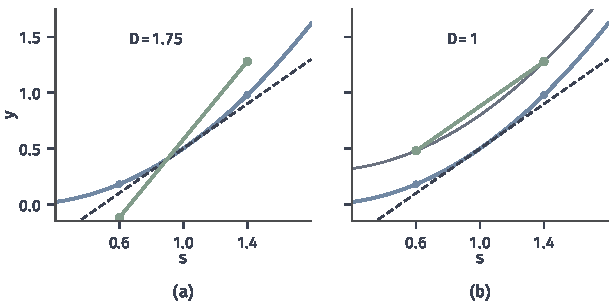
\includegraphics[width=104mm]{figures/05-optimization/05-stochastic-optimization/matplotlib/zo-pair-readings/figure.pdf}
  \caption{成对读数的两种接口，蓝线为$f(s)=s^2/2$，虚线是$s=1$处的切线，绿色线段连接两次读数，蓝点是真实函数值。(a)两点噪声独立，分别为$+0.3$和$-0.3$，线段斜率$1.75$，偏离切线。(b)两点共享噪声$+0.3$，读数都落在灰色曲线上，斜率恰为$1$。}
  \label{fig:zo-pair-readings}
\end{BookInlineFigure}

所以误差界必须与实际接口匹配。文献和本章后面给出的速率都带着接口条件，表~\ref{tab:zo-interfaces}先列出本章要用到的四种情形，第~\ref{sec:zo-pair-noise}节再推导对应的方差。

\begin{BookInlineTable}
  \centering
  \begin{tabular}{@{}lll@{}}
    \toprule
    接口 & 一轮读数 & 两点之差的噪声\\
    \midrule
    精确函数值 & 任意 & 无\\
    单点，含噪 & $1$ & 不适用\\
    成对，独立噪声 & $2$ & 方差$2\sigma^2$，不随距离变小\\
    成对，共享样本 & $2$ & 取决于样本函数的波动\\
    \bottomrule
  \end{tabular}
  \caption{本章区分的查询接口。“独立噪声”指式~\eqref{eq:zo-independent-pair}，噪声方差为$\sigma^2$；“共享样本”指式~\eqref{eq:zo-shared-pair}。}
  \label{tab:zo-interfaces}
\end{BookInlineTable}

\section{有限差分}
\label{sec:zo-finite-differences}

只凭几个函数值，怎样得到梯度的近似？思路来自一元微积分：导数是割线斜率的极限，步子小一点，割线斜率就接近导数。

\paragraph{从一元差商开始}
设$\varphi(s)$是一元函数，$h>0$是\term{扰动尺度}（perturbation scale）。两种常用的\term{差商}（difference quotient）是\term{前向差分}（forward difference）和\term{中心差分}（central difference）：
\begin{equation}
 \frac{\varphi(s+h)-\varphi(s)}{h},\qquad
 \frac{\varphi(s+h)-\varphi(s-h)}{2h}.
 \label{eq:zo-quotients-1d}
\end{equation}
图~\ref{fig:zo-secants}用$\varphi(s)=s^2/2+s^3/6$，$s_0=1$，$h=0.8$画出两条割线和切线。切线斜率是$\varphi'(1)=1.5$。

由$\varphi(1)=2/3$、$\varphi(1.8)=2.592$和$\varphi(0.2)\approx0.0213$，两种差商是
\[
 \frac{2.592-0.6667}{0.8}\approx2.407,\qquad
 \frac{2.592-0.0213}{1.6}\approx1.607.
\]
前向差商偏离$0.907$，中心差商只偏离$0.107$。原因是Taylor展开的二次项：前向割线把弯曲全部算进了斜率，中心割线的两侧弯曲互相抵消。

\begin{BookInlineFigure}
  \centering
  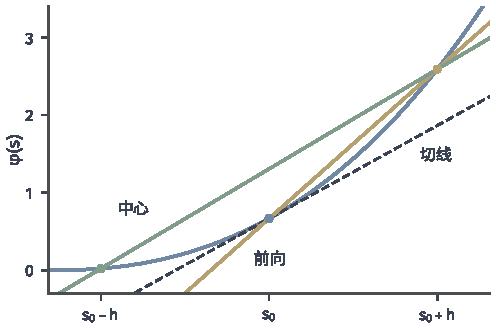
\includegraphics[width=84mm]{figures/05-optimization/05-stochastic-optimization/matplotlib/zo-secants/figure.pdf}
  \caption{$\varphi(s)=s^2/2+s^3/6$（蓝线）在$s_0=1$处的两种差商，$h=0.8$。虚线是切线，斜率$1.5$；黄线是前向割线，斜率约$2.407$；绿线是中心割线，斜率约$1.607$，方向最接近切线。}
  \label{fig:zo-secants}
\end{BookInlineFigure}

\paragraph{多元函数：沿一个方向看}
差商搬到多元函数上，只要限制在一条直线上。令$\varphi(s)=f(\bm{x}+s\bm{u})$，由链式法则$\varphi'(0)=\langle\nabla f(\bm{x}),\bm{u}\rangle$，这是方向导数。于是沿$\bm{u}$的中心差商近似$\langle\nabla f(\bm{x}),\bm{u}\rangle$。一次差商只告诉我们梯度在一个方向上的投影，要拼出整个梯度，需要多个方向，或者后面将看到的随机化。

下面的引理量化差商的\term{截断误差}（truncation error），它只涉及函数本身，不涉及噪声。第~\ref{chap:smooth-foundations}章的下降引理给出：$\nabla f$是$L$-Lipschitz时，对任意$\bm{x},\bm{v}$，
\[
 \bigl\lvert f(\bm{x}+\bm{v})-f(\bm{x})-\langle\nabla f(\bm{x}),\bm{v}\rangle\bigr\rvert
 \leq\frac{L}{2}\lVert\bm{v}\rVert_2^2.
\]

\begin{lemma}[差商的余项]
\label{lem:zo-remainder}
设$\nabla f$是$L$-Lipschitz的。对任意$\bm{x},\bm{v}$，
\begin{equation}
 \bigl\lvert f(\bm{x}+\bm{v})-f(\bm{x}-\bm{v})-2\langle\nabla f(\bm{x}),\bm{v}\rangle\bigr\rvert
 \leq L\lVert\bm{v}\rVert_2^2.
 \label{eq:zo-central-L}
\end{equation}
若$f$还二阶连续可微，且$\nabla^2f$按谱范数是$M$-Lipschitz的，则
\begin{equation}
 \bigl\lvert f(\bm{x}+\bm{v})-f(\bm{x}-\bm{v})-2\langle\nabla f(\bm{x}),\bm{v}\rangle\bigr\rvert
 \leq\frac{M}{3}\lVert\bm{v}\rVert_2^3.
 \label{eq:zo-central-M}
\end{equation}
\end{lemma}

\begin{proof}
把上面的不等式分别用于$\bm{v}$和$-\bm{v}$，两式相减，由三角不等式得式~\eqref{eq:zo-central-L}。

对第二个结论，记$\bm{H}=\nabla^2f(\bm{x})$。积分形式的Taylor公式给出
\[
 \begin{aligned}
 &f(\bm{x}+\bm{v})-f(\bm{x})-\langle\nabla f(\bm{x}),\bm{v}\rangle-\frac12\bm{v}^\top\bm{H}\bm{v}\\
 &\quad=\int_0^1(1-s)\,\bm{v}^\top\bigl(\nabla^2f(\bm{x}+s\bm{v})-\bm{H}\bigr)\bm{v}\,\mathrm{d}s.
 \end{aligned}
\]
右端的绝对值不超过
\[
 \int_0^1(1-s)\,Ms\,\lVert\bm{v}\rVert_2^3\,\mathrm{d}s=\frac{M}{6}\lVert\bm{v}\rVert_2^3.
\]
对$\bm{v}$和$-\bm{v}$各写一次再相减，二次项$\tfrac12\bm{v}^\top\bm{H}\bm{v}$恰好相消，余项相加得$\tfrac{M}{3}\lVert\bm{v}\rVert_2^3$。
\end{proof}

\paragraph{三笔账}
每种差分都要记三笔账。第一笔是截断误差，随$h$变小而变小。第二笔是读数噪声造成的误差：独立噪声方差$\sigma^2$时，前向差商的噪声是$(\zeta_1-\zeta_0)/h$，中心差商的噪声是$(\zeta_+-\zeta_-)/(2h)$，方差分别为
\begin{equation}
 \frac{2\sigma^2}{h^2},\qquad\frac{\sigma^2}{2h^2},
 \label{eq:zo-quotient-noise}
\end{equation}
都随$h$变小而变大。第三笔是查询次数。这三笔账彼此独立，下面逐个方法记录，第~\ref{sec:zo-tradeoff}节再做取舍。

\subsection{坐标差分}
\label{sec:zo-coordinate}

最直接的做法是沿$n$个坐标方向逐个差分，用$n$个方向导数拼成梯度。记$\bm{e}_i$为第$i$个标准基向量，两种\term{坐标差分}（coordinate difference）的第$i$个分量是
\begin{equation}
 \hat{g}^{\mathrm{F}}_i=\frac{f(\bm{x}+h\bm{e}_i)-f(\bm{x})}{h},\qquad
 \hat{g}^{\mathrm{C}}_i=\frac{f(\bm{x}+h\bm{e}_i)-f(\bm{x}-h\bm{e}_i)}{2h}.
 \label{eq:zo-coordinate}
\end{equation}

\paragraph{查询次数}
前向差分的$n$个分量可以共用中心读数$f(\bm{x})$，所以一共$n+1$次查询。中心差分每个坐标读两点，共$2n$次，中心点本身不读。图~\ref{fig:zo-stencils}(a)(b)画出了这两种查询模式。

\begin{BookInlineFigure}
  \centering
  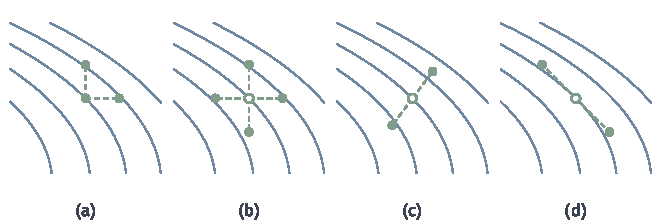
\includegraphics[width=112mm]{figures/05-optimization/05-stochastic-optimization/matplotlib/zo-stencils/figure.pdf}
  \caption{贯穿例在$(9,1)$附近的查询点，蓝线是等高线，为便于观察取$h=0.4$。实心点要读函数值，空心点是当前点、不读。(a)前向坐标差分，$3$次。(b)中心坐标差分，$4$次。(c)沿$\bm{u}=(0.6,0.8)$的随机方向差分，$2$次。(d)第~\ref{sec:zo-spsa}节的同时扰动，$\bm{\Delta}=(1,-1)$，$2$次，位移长度是$h\sqrt{2}$。}
  \label{fig:zo-stencils}
\end{BookInlineFigure}

\paragraph{手算比较}
在贯穿例的起点取$h=0.1$。为算前向差商，读三个函数值：
\[
 f(9,1)=45,\qquad f(9.1,1)=45.905,\qquad f(9,1.1)=45.945.
\]
代入式~\eqref{eq:zo-coordinate}，前向差分给出
\[
 \hat{\bm{g}}^{\mathrm{F}}=(9.05,\ 9.45).
\]
真实梯度是$(9,9)$，误差$(0.05,\,0.45)$，恰好等于$\tfrac{h}{2}H_{ii}$：沿$x_2$方向弯曲是$x_1$方向的$9$倍，误差也是$9$倍。

再读$f(8.9,1)=44.105$和$f(9,0.9)=44.145$，中心差分给出
\[
 \hat{\bm{g}}^{\mathrm{C}}=\Bigl(\frac{45.905-44.105}{0.2},\ \frac{45.945-44.145}{0.2}\Bigr)=(9,\ 9).
\]
对二次函数，中心差分没有截断误差，因为三阶以上的导数都是零。多付一次查询，换来了精确值。

\paragraph{截断误差的一般结论}
上面的现象对一般函数也成立，只是阶数要由相应的导数条件来保证。

\begin{theorem}[坐标差分的截断误差]
\label{thm:zo-coordinate}
设读数精确。若$\nabla f$是$L$-Lipschitz的，则
\begin{equation}
 \lVert\hat{\bm{g}}^{\mathrm{F}}-\nabla f(\bm{x})\rVert_2\leq\frac{\sqrt{n}\,Lh}{2}.
 \label{eq:zo-coordinate-forward}
\end{equation}
若$f$还二阶连续可微且$\nabla^2f$是$M$-Lipschitz的，则
\begin{equation}
 \lVert\hat{\bm{g}}^{\mathrm{C}}-\nabla f(\bm{x})\rVert_2\leq\frac{\sqrt{n}\,Mh^2}{6}.
 \label{eq:zo-coordinate-central}
\end{equation}
\end{theorem}

\begin{proof}
对前向差分，把下降引理用于$\bm{v}=h\bm{e}_i$，再除以$h$，得
\[
 \lvert\hat{g}^{\mathrm{F}}_i-\partial_if(\bm{x})\rvert\leq\frac{Lh}{2}.
\]

对中心差分，把式~\eqref{eq:zo-central-M}用于$\bm{v}=h\bm{e}_i$，再除以$2h$，得
\[
 \lvert\hat{g}^{\mathrm{C}}_i-\partial_if(\bm{x})\rvert\leq\frac{Mh^2}{6}.
\]
$n$个分量各不超过同一个上界，向量的欧氏范数不超过该上界乘以$\sqrt{n}$。
\end{proof}

定理的条件各有作用。前向差分只用到梯度的Lipschitz性，误差是一阶的。中心差分要快一阶，需要三阶信息受控，也就是Hessian的Lipschitz性；只有$L$时，由式~\eqref{eq:zo-central-L}只能得到每个分量$Lh/2$，与前向差分同阶。

图~\ref{fig:zo-trunc-log}在$\varphi(s)=s^2/2+s^3/6$上验证这两个阶数。双对数坐标下，前向误差的斜率是$1$，中心误差的斜率是$2$，$h$每缩小$10$倍，中心差分的误差缩小$100$倍。

\begin{BookInlineFigure}
  \centering
  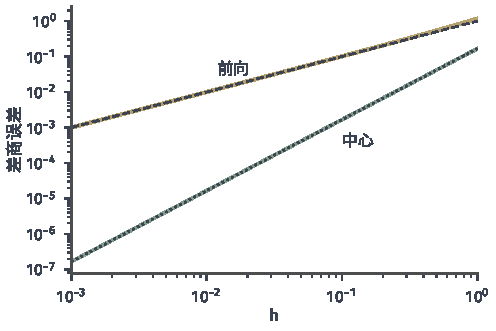
\includegraphics[width=84mm]{figures/05-optimization/05-stochastic-optimization/matplotlib/zo-trunc-log/figure.pdf}
  \caption{精确读数下差商误差随$h$的变化，$\varphi(s)=s^2/2+s^3/6$，$s_0=1$，真实导数$1.5$。黄线为前向差分，绿线为中心差分；虚线是$h$，点线是$h^2/6$，分别对应理论的斜率$1$和$2$。}
  \label{fig:zo-trunc-log}
\end{BookInlineFigure}

\subsection{随机方向差分}
\label{sec:zo-random-direction}

坐标差分每算一次梯度要$n$轮查询，维数大时一步也走不起。一个自然的想法是：每轮只沿一个方向差分，方向随机抽，多轮平均下来也许能覆盖各个方向。

\paragraph{从方向导数恢复向量}
一次差商是一个标量，要把它变成向量，乘上方向本身。设$\bm{u}$在单位球面$\bm{S}$（$\mathbb{R}^n$中全体长度为$1$的向量）上均匀分布。记$\bm{g}=\nabla f(\bm{x})$，考察$\langle\bm{g},\bm{u}\rangle\bm{u}$的均值。由对称性，$\mathbb{E}[u_iu_j]=0$（$i\neq j$），且$n$个$\mathbb{E}[u_i^2]$相等，和为$1$，所以
\[
 \mathbb{E}[\bm{u}\bm{u}^\top]=\frac{1}{n}\bm{I}.
\]
于是
\[
 \mathbb{E}\bigl[\langle\bm{g},\bm{u}\rangle\bm{u}\bigr]=\mathbb{E}[\bm{u}\bm{u}^\top]\bm{g}=\frac{1}{n}\bm{g}.
\]
乘以$n$就得到$\bm{g}$的无偏量。把方向导数换成中心差商，定义\term{随机方向差分}（random-direction difference）：
\begin{equation}
 D_h(\bm{u})=\frac{f(\bm{x}+h\bm{u})-f(\bm{x}-h\bm{u})}{2h},\qquad
 \hat{\bm{g}}=n\,D_h(\bm{u})\,\bm{u}.
 \label{eq:zo-random-direction}
\end{equation}
一般地，若方向分布满足$\mathbb{E}[\bm{u}\bm{u}^\top]=c\,\bm{I}$，归一化因子就是$1/c$。因子$n$来自单位球面的二阶矩，不是万能常数。

\paragraph{一条方向只有一条方向的信息}
在起点，贯穿例是二次函数，中心差商精确等于方向导数，$\hat{\bm{g}}=2\langle\bm{g},\bm{u}\rangle\bm{u}$。取几个方向，结果如下：
\[
 \bm{u}=(1,0):\ \hat{\bm{g}}=(18,0),\qquad
 \bm{u}=(0,1):\ \hat{\bm{g}}=(0,18).
\]
第三、第四个方向是$(1,1)/\sqrt{2}$和$(1,-1)/\sqrt{2}$，得到
\[
 \hat{\bm{g}}=(18,18),\qquad\hat{\bm{g}}=(0,0).
\]
四个估计的平均是$(9,9)$，但没有一个单独接近$(9,9)$。方向$(1,-1)/\sqrt{2}$与梯度垂直，一条差商得到零，什么也看不出来。

图~\ref{fig:zo-circle}(a)说明所有估计的分布：$n=2$时，$2\langle\bm{g},\bm{u}\rangle\bm{u}$走遍一个以$\bm{g}$为圆心、过原点的圆。圆心就是均值，半径就是误差的大小。单个估计总是偏离$\lVert\bm{g}\rVert_2$，只有平均才接近$\bm{g}$。

\begin{BookInlineFigure}
  \centering
  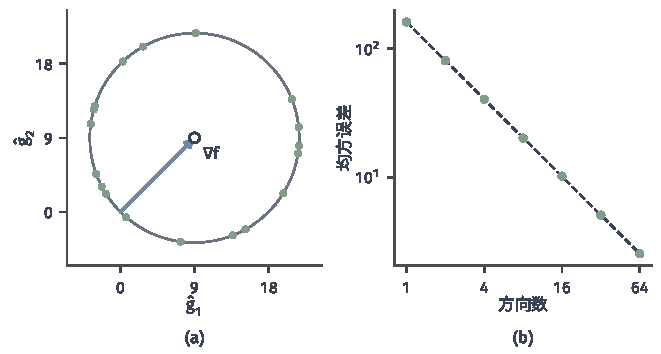
\includegraphics[width=112mm]{figures/05-optimization/05-stochastic-optimization/matplotlib/zo-circle/figure.pdf}
  \caption{贯穿例起点处$\bm{g}=(9,9)$的随机方向估计。(a)绿点是$18$个随机方向给出的$2\langle\bm{g},\bm{u}\rangle\bm{u}$，全部落在以$\bm{g}$（空心圆）为圆心、半径$\lVert\bm{g}\rVert_2$的灰圆上，蓝色箭头是真实梯度。(b)$m$个独立方向平均后的均方误差，绿点是Monte Carlo结果，虚线是$162/m$。}
  \label{fig:zo-circle}
\end{BookInlineFigure}

\paragraph{偏差与二阶矩}
下面的定理把偏差和波动分开。

\begin{theorem}[随机方向差分]
\label{thm:zo-random-direction}
设读数精确，$\bm{u}$在$\bm{S}$上均匀分布，$\hat{\bm{g}}$由式~\eqref{eq:zo-random-direction}定义。若$f$是二次函数，则
\begin{equation}
 \mathbb{E}[\hat{\bm{g}}]=\bm{g},\qquad
 \mathbb{E}\lVert\hat{\bm{g}}-\bm{g}\rVert_2^2=(n-1)\lVert\bm{g}\rVert_2^2.
 \label{eq:zo-direction-quadratic}
\end{equation}
若$f$二阶连续可微且$\nabla^2f$是$M$-Lipschitz的，则偏差满足
\begin{equation}
 \bigl\lVert\mathbb{E}[\hat{\bm{g}}]-\bm{g}\bigr\rVert_2\leq\frac{nMh^2}{6}.
 \label{eq:zo-direction-bias}
\end{equation}
\end{theorem}

\begin{proof}
二次函数的中心差商没有余项，$\hat{\bm{g}}=n\langle\bm{g},\bm{u}\rangle\bm{u}$，由$\mathbb{E}[\bm{u}\bm{u}^\top]=\bm{I}/n$得$\mathbb{E}[\hat{\bm{g}}]=\bm{g}$。

二阶矩用$\lVert\bm{u}\rVert_2=1$计算：
\[
 \mathbb{E}\lVert\hat{\bm{g}}\rVert_2^2=n^2\mathbb{E}\langle\bm{g},\bm{u}\rangle^2=n^2\cdot\frac{\lVert\bm{g}\rVert_2^2}{n}=n\lVert\bm{g}\rVert_2^2.
\]
减去均值的平方$\lVert\bm{g}\rVert_2^2$，得到方差。

一般情形写$D_h(\bm{u})=\langle\bm{g},\bm{u}\rangle+r$。把式~\eqref{eq:zo-central-M}用于$\bm{v}=h\bm{u}$并除以$2h$，得$\lvert r\rvert\leq Mh^2/6$。于是
\[
 \bigl\lVert\mathbb{E}[\hat{\bm{g}}]-\bm{g}\bigr\rVert_2=n\bigl\lVert\mathbb{E}[r\bm{u}]\bigr\rVert_2\leq n\,\mathbb{E}\lvert r\rvert\leq\frac{nMh^2}{6}.
\]
\end{proof}

式~\eqref{eq:zo-direction-quadratic}的$n-1$就是维数的代价：一条方向只探测了$n$维中的一维，其余$n-1$维的信息要靠多轮平均。图~\ref{fig:zo-circle}(b)验证了$m$个独立方向平均后，均方误差按$(n-1)\lVert\bm{g}\rVert_2^2/m$下降。

\paragraph{有限扰动下一般有偏}
二次函数上的无偏是特例。一旦有三阶项，中心差商不再等于方向导数，由它乘$\bm{u}$形成的向量，均值一般不等于原梯度。取$n=2$，$f(\bm{x})=x_1^3$，在$x_1=0$处真实梯度为零。差商和估计为
\[
 D_h(\bm{u})=h^2u_1^3,\qquad\hat{\bm{g}}=2h^2u_1^3\,\bm{u}.
\]
记$\bm{u}=(\cos\theta,\sin\theta)$。由$\mathbb{E}[\cos^4\theta]=\tfrac38$和$\mathbb{E}[\cos^3\theta\sin\theta]=0$，
\[
 \mathbb{E}[\hat{\bm{g}}]=\bigl(\tfrac34h^2,\ 0\bigr)\neq\bm{0}.
\]
这里$M=6$，定理的界是$2h^2$，实际偏差$\tfrac34h^2$在界内。偏差确实存在，而且随$h$平方缩小。

\subsection{同时扰动随机逼近}
\label{sec:zo-spsa}

随机方向差分要从球面上抽方向，并且需要因子$n$。Spall提出的\term{同时扰动随机逼近}（simultaneous perturbation stochastic approximation，SPSA）用更简单的方式达到类似的效果：让所有坐标同时动一下，每个坐标只取正负两个方向。

\paragraph{主要思想}
抽取向量$\bm{\Delta}\in\{-1,+1\}^n$，各分量独立，等可能取$\pm1$。查询两点$\bm{x}\pm h\bm{\Delta}$，算一个函数差，再把同一个差除以各分量的扰动：
\begin{equation}
 D=\frac{y_+-y_-}{2h},\qquad \hat{g}_i=\frac{D}{\Delta_i},\quad i=1,\ldots,n.
 \label{eq:zo-spsa}
\end{equation}
只读了两次，却得到了$n$个分量。为什么这样能行？若$f$是二次函数，$D=\langle\bm{g},\bm{\Delta}\rangle$，于是
\[
 \hat{g}_i=g_i+\sum_{j\neq i}g_j\frac{\Delta_j}{\Delta_i}.
\]
第一项是想要的。后面每一项都是其他坐标的“串扰”。因为$\Delta_j$与$\Delta_i$独立，且$\mathbb{E}[\Delta_j]=0$，串扰的均值是零，平均之后消失。

除法要求$\mathbb{E}[1/\lvert\Delta_i\rvert]$有限，这解释了分布的选择。正态或区间上的均匀扰动在$0$附近有正的密度，$1/\lvert\Delta_i\rvert$的期望发散，不能用于这个公式。$\pm1$时$1/\Delta_i=\Delta_i$，估计也可以写成$\hat{\bm{g}}=D\,\bm{\Delta}$。

\paragraph{手算四种情形}
贯穿例起点，$h=0.1$，$n=2$，$\bm{\Delta}$有四种等可能取值。取$\bm{\Delta}=(1,1)$，读数和差商是
\[
 y_+=f(9.1,1.1)=46.85,\qquad y_-=f(8.9,0.9)=43.25,\qquad D=18.
\]
取$\bm{\Delta}=(1,-1)$，两次读数相等，差商为零：
\[
 y_+=f(9.1,0.9)=45.05,\qquad y_-=f(8.9,1.1)=45.05,\qquad D=0.
\]
$-\bm{\Delta}$与$\bm{\Delta}$的结果相同。四种情形的估计分别是$(18,18)$、$(0,0)$、$(0,0)$、$(18,18)$，平均恰为$(9,9)$，如图~\ref{fig:zo-spsa}(b)。

\begin{BookInlineFigure}
  \centering
  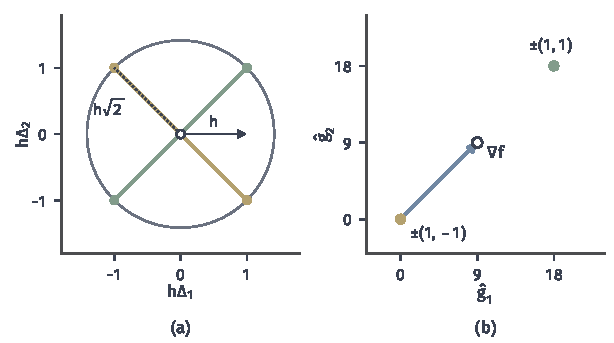
\includegraphics[width=104mm]{figures/05-optimization/05-stochastic-optimization/matplotlib/zo-spsa/figure.pdf}
  \caption{$n=2$时的同时扰动。(a)四个扰动$h\bm{\Delta}$（$h=1$）位于正方形顶点，一对相反的点共用一次差分，绿、黄各一对；每个坐标只动$h$，位移长度却是$h\sqrt{2}$，四点都在半径$h\sqrt{2}$的圆上。(b)贯穿例起点的估计，绿点是$\bm{\Delta}=\pm(1,1)$的结果，黄点是$\bm{\Delta}=\pm(1,-1)$的结果，它们的平均是真实梯度（空心圆）。}
  \label{fig:zo-spsa}
\end{BookInlineFigure}

\paragraph{偏差与噪声}
SPSA在原梯度上的偏差由差商余项决定，与随机方向差分的结论形式一样，只是这里的位移长度不再是$h$。

\begin{theorem}[SPSA的偏差]
\label{thm:zo-spsa}
设$f$二阶连续可微，$\nabla^2f$是$M$-Lipschitz的，$\bm{\Delta}$的分量独立且等可能取$\pm1$，读数为$y_\pm=f(\bm{x}\pm h\bm{\Delta})+\zeta_\pm$，且给定$\bm{x},\bm{\Delta}$时$\zeta_+-\zeta_-$的条件均值为零。则对$\hat{\bm{g}}$的每个分量，
\begin{equation}
 \bigl\lvert\mathbb{E}[\hat{g}_i\mid\bm{x}]-\partial_if(\bm{x})\bigr\rvert\leq\frac{M h^2n^{3/2}}{6}.
 \label{eq:zo-spsa-bias}
\end{equation}
\end{theorem}

\begin{proof}
$\lVert h\bm{\Delta}\rVert_2=h\sqrt{n}$。把差商写成主项、余项和噪声三部分：
\[
 D=\langle\bm{g},\bm{\Delta}\rangle+r+\frac{\zeta_+-\zeta_-}{2h}.
\]
由式~\eqref{eq:zo-central-M}，余项满足
\[
 \lvert r\rvert\leq\frac{1}{2h}\cdot\frac{M}{3}(h\sqrt{n})^3=\frac{Mh^2n^{3/2}}{6}.
\]
除以$\Delta_i$后取条件期望。主项由串扰的零均值给出$g_i$；噪声项先对给定的$\bm{\Delta}$取期望，为零；余项的绝对值不变，因为$\lvert\Delta_i\rvert=1$。
\end{proof}

对二次函数$r=0$，SPSA精确无偏。一般函数上$h$有限时仍有偏差，只有$h\to0$时偏差才消失，这一点与随机方向差分相同。定理只要求噪声差的条件均值为零，噪声本身不必独立。

\paragraph{坐标尺度与位移长度}
比较SPSA和球面方向时容易犯一个错误：SPSA的$h$是每个坐标的扰动，实际位移长度是$h\sqrt{n}$。在$n=100$、$h=0.1$时，查询点已偏离当前点$1$个单位。公平的比较要令位移长度相同，取$h=\delta/\sqrt{n}$与球面半径$\delta$对应。

这样比较之后两者的噪声完全一致。独立噪声下，SPSA的$\lVert\hat{\bm{g}}\rVert_2^2$中噪声贡献的均值是$n\sigma^2/(2h^2)$，代入$h=\delta/\sqrt{n}$得
\[
 \frac{n^2\sigma^2}{2\delta^2},
\]
恰好等于球面方向的噪声贡献$n^2\cdot\sigma^2/(2\delta^2)$。二次函数上，SPSA的二阶矩也与球面方向相同：
\[
 \mathbb{E}\lVert\hat{\bm{g}}\rVert_2^2=n\,\mathbb{E}\langle\bm{g},\bm{\Delta}\rangle^2=n\lVert\bm{g}\rVert_2^2.
\]
SPSA的优势主要在实现简单，每个坐标扰动大小固定。

表~\ref{tab:zo-differences}汇总本节三种差分。

\begin{BookInlineTable}
  \centering
  \begin{tabular}{@{}llll@{}}
    \toprule
    方法 & 查询 & 截断偏差 & 独立噪声的二阶矩\\
    \midrule
    前向坐标 & $n+1$ & $\sqrt{n}Lh/2$ & $2n\sigma^2/h^2$\\
    中心坐标 & $2n$ & $\sqrt{n}Mh^2/6$ & $n\sigma^2/(2h^2)$\\
    随机方向 & $2$ & $nMh^2/6$ & $n^2\sigma^2/(2h^2)$\\
    SPSA & $2$ & $n^2Mh^2/6$ & $n\sigma^2/(2h^2)$\\
    \bottomrule
  \end{tabular}
  \caption{三种差分的成本与误差。偏差为欧氏范数的上界，SPSA一行由式~\eqref{eq:zo-spsa-bias}乘$\sqrt{n}$得到。独立噪声的二阶矩指$\mathbb{E}\lVert\text{噪声造成的估计误差}\rVert_2^2$，SPSA的$h$是坐标尺度，位移长度为$h\sqrt{n}$。}
  \label{tab:zo-differences}
\end{BookInlineTable}

\section{随机平滑与梯度估计}
\label{sec:zo-smoothing}

上一节的估计以原梯度为目标，有限的$h$总带来偏差。于是要问：能否换一个目标，让函数值给出的估计严格无偏？答案是把目标函数在一个小邻域上取平均。平均之后的函数有自己的梯度，而这个梯度恰好可以写成函数值的期望。

打个比方，用原目标比较两点的高低，好比踩着一块小石头判断地面坡度，容易被局部起伏误导；平滑目标则像站在一块平板上，平板的倾斜由它覆盖的整片地面决定。我们估计的是平板的倾斜，不是脚下那一点的坡度。比方的边界也要记住：平板的倾斜和地面的坡度是两个对象，它们的差别要到第~\ref{sec:zo-original-error}节才算清。

\subsection{平滑目标}
\label{sec:zo-smooth-target}

\paragraph{定义}
记$\bm{B}$为$\mathbb{R}^n$中的单位球，即全体长度不超过$1$的向量。下面给出两种平均方式，$\delta>0$是球的半径，$\tau>0$是高斯分布的尺度。

\begin{definition}[球平滑与高斯平滑]
\label{def:zo-smoothing}
设$\bm{v}$在$\bm{B}$上均匀分布，$\bm{w}\sim\mathcal{N}(\bm{0},\bm{I})$。$f$的\term{球平滑}（ball smoothing）与\term{高斯平滑}（Gaussian smoothing）分别是
\begin{equation}
 f^{\mathrm{B}}_{\delta}(\bm{x})=\mathbb{E}_{\bm{v}}\bigl[f(\bm{x}+\delta\bm{v})\bigr],\qquad
 f^{\mathrm{G}}_{\tau}(\bm{x})=\mathbb{E}_{\bm{w}}\bigl[f(\bm{x}+\tau\bm{w})\bigr].
 \label{eq:zo-smoothing}
\end{equation}
前提是期望有定义。它们统称\term{平滑目标}（smoothed objective）。
\end{definition}

\paragraph{定义成立需要什么}
两种平均对$f$的要求不同。球平滑只看$\bm{x}$周围半径$\delta$的球，$f$在这个球上局部可积就够了，比如局部连续。它对球外的$f$没有任何要求。

高斯平滑要看整个空间，于是必须控制$f$在无穷远的增长，局部的好性质帮不上忙。例如$n=1$，$f(x)=e^{x^2}$处处光滑，但
\[
 \mathbb{E}\bigl[e^{(x+\tau w)^2}\bigr]<\infty\quad\Longleftrightarrow\quad 2\tau^2<1.
\]
$\tau\geq1/\sqrt{2}$时高斯平滑根本不存在。多项式增长或指数增长（$\lvert f(\bm{z})\rvert$不超过$Ce^{a\lVert\bm{z}\rVert_2}$）都可以被高斯密度压住。

\paragraph{二次函数上的平滑}
贯穿例上平滑的效果可以算出来。二次函数满足
\[
 f(\bm{x}+\bm{z})=f(\bm{x})+\langle\nabla f(\bm{x}),\bm{z}\rangle+\frac12\bm{z}^\top\bm{H}\bm{z}.
\]
取$\bm{z}$为对称分布的扰动，一次项的期望为零。均匀球上$\mathbb{E}[\bm{v}\bm{v}^\top]=\bm{I}/(n+2)$，所以
\[
 f^{\mathrm{B}}_{\delta}(\bm{x})=f(\bm{x})+\frac{\delta^2\operatorname{tr}\bm{H}}{2(n+2)},\qquad
 f^{\mathrm{G}}_{\tau}(\bm{x})=f(\bm{x})+\frac{\tau^2\operatorname{tr}\bm{H}}{2}.
\]
贯穿例$\operatorname{tr}\bm{H}=10$，$n=2$，分别得到$f+1.25\delta^2$和$f+5\tau^2$。平滑只把目标抬高一个常数，梯度完全不变。所以在二次函数上，平滑目标的梯度就是原梯度，这也解释了上一节的中心差分为什么在二次函数上无偏。

\paragraph{绝对值函数：不可微时平滑仍可微}
平滑真正的用处在不光滑的目标上。$f(x)=\lvert x\rvert$在$0$处没有导数。$n=1$时单位球是区间$[-1,1]$，直接积分得到
\begin{equation}
 f^{\mathrm{B}}_{\delta}(x)=
 \begin{cases}
 \dfrac{x^2+\delta^2}{2\delta},&\lvert x\rvert\leq\delta,\\
 \lvert x\rvert,&\lvert x\rvert>\delta.
 \end{cases}
 \label{eq:zo-abs-ball}
\end{equation}
它的导数在$\lvert x\rvert\leq\delta$上是$x/\delta$，在$x=\pm\delta$处与外侧的$\pm1$衔接，因此连续可微。高斯平滑的结果用误差函数表示：
\[
 f^{\mathrm{G}}_{\tau}(x)=\tau\sqrt{\frac{2}{\pi}}\,e^{-x^2/(2\tau^2)}+x\operatorname{erf}\Bigl(\frac{x}{\sqrt{2}\tau}\Bigr).
\]
图~\ref{fig:zo-smooth-abs}取$\delta=1$，$\tau=1/\sqrt{3}$，这时两种扰动的方差相同。尖点被磨圆了，但代价也在图上：$x=0$处，两条曲线的值分别是$1/2$和约$0.46$，原函数值是$0$。

\begin{BookInlineFigure}
  \centering
  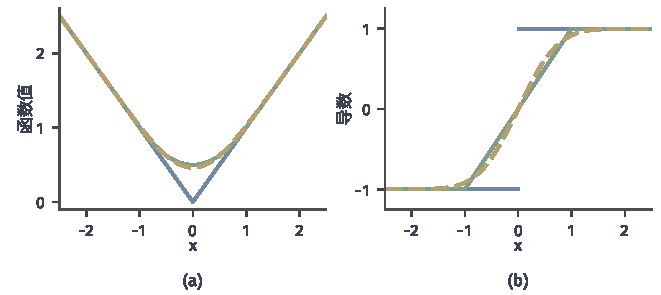
\includegraphics[width=112mm]{figures/05-optimization/05-stochastic-optimization/matplotlib/zo-smooth-abs/figure.pdf}
  \caption{$f(x)=\lvert x\rvert$的平滑。蓝线是原函数，绿线是$\delta=1$的球平滑，黄色虚线是$\tau=1/\sqrt{3}$的高斯平滑。(a)函数值，尖点被磨圆且抬高。(b)导数，原函数在$0$处跳变，平滑后连续。}
  \label{fig:zo-smooth-abs}
\end{BookInlineFigure}

\paragraph{平滑误差}
平滑目标与原目标差多少，由原目标的光滑程度决定。下面的引理后面会多次使用。

\begin{lemma}[平滑的基本性质]
\label{lem:zo-smoothing-properties}
\begin{enumerate}
 \item 若$\nabla f$是$L$-Lipschitz的，则$f^{\mathrm{B}}_{\delta}$与$f^{\mathrm{G}}_{\tau}$的梯度也是$L$-Lipschitz的，并且
 \begin{equation}
  \lvert f^{\mathrm{B}}_{\delta}-f\rvert\leq\frac{L\delta^2}{2},\qquad
  \lVert\nabla f^{\mathrm{B}}_{\delta}-\nabla f\rVert_2\leq L\delta,
  \label{eq:zo-ball-error}
 \end{equation}
 \begin{equation}
  \lvert f^{\mathrm{G}}_{\tau}-f\rvert\leq\frac{L\tau^2n}{2},\qquad
  \lVert\nabla f^{\mathrm{G}}_{\tau}-\nabla f\rVert_2\leq L\tau\sqrt{n}.
  \label{eq:zo-gauss-error}
 \end{equation}
 \item 若$f$是$G$-Lipschitz的，则
 \begin{equation}
  \lvert f^{\mathrm{B}}_{\delta}-f\rvert\leq G\delta.
  \label{eq:zo-lipschitz-error}
 \end{equation}
 \item 若$f$是凸函数，则平滑目标也是凸函数，且$f^{\mathrm{B}}_{\delta}\geq f$，$f^{\mathrm{G}}_{\tau}\geq f$。
\end{enumerate}
\end{lemma}

\begin{proof}
只写球平滑，高斯平滑把$\delta\bm{v}$换成$\tau\bm{w}$，并用$\mathbb{E}\lVert\bm{w}\rVert_2^2=n$与$\mathbb{E}\lVert\bm{w}\rVert_2\leq\sqrt{n}$。

第一项。$\nabla f$连续且至多线性增长，可在期望号下求导：
\[
 \nabla f^{\mathrm{B}}_{\delta}(\bm{x})=\mathbb{E}\bigl[\nabla f(\bm{x}+\delta\bm{v})\bigr].
\]
两点作差，由$\nabla f$的Lipschitz性得到相同常数$L$。由$\mathbb{E}[\bm{v}]=\bm{0}$，
\[
 f^{\mathrm{B}}_{\delta}(\bm{x})-f(\bm{x})=\mathbb{E}\bigl[f(\bm{x}+\delta\bm{v})-f(\bm{x})-\delta\langle\nabla f(\bm{x}),\bm{v}\rangle\bigr].
\]
下降引理给出右端绝对值不超过
\[
 \frac{L}{2}\delta^2\,\mathbb{E}\lVert\bm{v}\rVert_2^2\leq\frac{L\delta^2}{2}.
\]
梯度差由$\nabla f$的Lipschitz性取期望，不超过$L\delta$。

第二项由下式取期望得到：
\[
 \lvert f(\bm{x}+\delta\bm{v})-f(\bm{x})\rvert\leq G\delta\lVert\bm{v}\rVert_2\leq G\delta.
\]

第三项。对每个固定的$\bm{v}$，$\bm{x}\mapsto f(\bm{x}+\delta\bm{v})$是凸函数，凸函数的平均是凸函数。再由Jensen不等式：凸函数在随机点上的平均不小于在平均点上的值，
\[
 f^{\mathrm{B}}_{\delta}(\bm{x})=\mathbb{E}[f(\bm{x}+\delta\bm{v})]\geq f\bigl(\bm{x}+\delta\mathbb{E}[\bm{v}]\bigr)=f(\bm{x}).
\]
\end{proof}

式~\eqref{eq:zo-gauss-error}比式~\eqref{eq:zo-ball-error}多了维数因子。这不是高斯平滑更差，而是$\tau$的含义不同：$\tau\bm{w}$的长度约为$\tau\sqrt{n}$。令$\tau=\delta/\sqrt{n}$时，两组界同阶。

\subsection{单点估计}
\label{sec:zo-one-point}

现在寻找用函数值表示平滑梯度的公式。出发点是一个几何观察，图~\ref{fig:zo-disc-shift}画的是$n=2$的情形。

\paragraph{主要思想}
把球心从$\bm{x}$移动一点点到$\bm{x}+\Delta\bm{x}$，球内积分的变化只发生在边界：右边新进入一片月牙，左边离开一片月牙，中间的部分原封不动。所以球平均的变化率完全由球面上的函数值决定，球内部的值只通过边界起作用。

把这个想法写成式子。月牙在法向$\bm{u}$处的厚度是$\langle\Delta\bm{x},\bm{u}\rangle$，于是积分的一阶变化是球面积分$\int f(\bm{x}+\delta\bm{u})\langle\Delta\bm{x},\bm{u}\rangle\,\mathrm{d}S$。再除以球的体积。半径$\delta$的球面积与球体积之比是$n/\delta$，这就是公式里因子的来历。

\begin{BookInlineFigure}
  \centering
  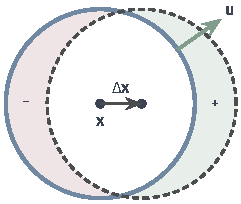
\includegraphics[width=41mm]{figures/05-optimization/05-stochastic-optimization/tikz/zo-disc-shift/figure.pdf}
  \caption{球平滑梯度的来历。蓝色实线是以$\bm{x}$为心的圆，虚线是平移$\Delta\bm{x}$后的圆。绿色月牙是新进入的区域，红色月牙是离开的区域，公共部分对积分的变化没有贡献。月牙在外法向$\bm{u}$处的厚度约为$\langle\Delta\bm{x},\bm{u}\rangle$。}
  \label{fig:zo-disc-shift}
\end{BookInlineFigure}

\begin{theorem}[球平滑的梯度恒等式]
\label{thm:zo-ball-identity}
设$f$在开集$\bm{U}$上连续，闭球$\bm{x}+\delta\bm{B}\subset\bm{U}$，$\bm{u}$在单位球面$\bm{S}$上均匀分布。则$f^{\mathrm{B}}_{\delta}$在$\bm{x}$处可微，且
\begin{equation}
 \nabla f^{\mathrm{B}}_{\delta}(\bm{x})=\frac{n}{\delta}\,\mathbb{E}_{\bm{u}}\bigl[f(\bm{x}+\delta\bm{u})\,\bm{u}\bigr].
 \label{eq:zo-ball-identity}
\end{equation}
\end{theorem}

\begin{proof}
先设$f$连续可微。可在积分号下求导，得
\[
 \partial_if^{\mathrm{B}}_{\delta}(\bm{x})=\frac{1}{\operatorname{vol}(\delta\bm{B})}\int_{\delta\bm{B}}\partial_if(\bm{x}+\bm{z})\,\mathrm{d}\bm{z}.
\]
对向量场$f(\bm{x}+\bm{z})\bm{e}_i$在球$\delta\bm{B}$上用散度定理，外法向是$\bm{z}/\delta$，于是
\[
 \partial_if^{\mathrm{B}}_{\delta}(\bm{x})=\frac{1}{\operatorname{vol}(\delta\bm{B})}\int_{\delta\bm{S}}f(\bm{x}+\bm{z})\frac{z_i}{\delta}\,\mathrm{d}S(\bm{z}).
\]

半径$\delta$的球体积是$c\,\delta^n$，对半径求导得球面积$nc\,\delta^{n-1}$，两者之比为$n/\delta$。把球面积分写成均匀分布下的期望，$\bm{z}=\delta\bm{u}$，就得到式~\eqref{eq:zo-ball-identity}。

再设$f$只连续。取$\bm{x}$的一个小邻域，使它的$\delta$膨胀的闭包是$\bm{U}$内的紧集，用光滑函数$f_k$在这个紧集上一致逼近$f$。$f_k$的平滑函数一致收敛到$f^{\mathrm{B}}_{\delta}$，它们的梯度由恒等式给出，一致收敛到式~\eqref{eq:zo-ball-identity}右端，右端关于位置连续。函数列一致收敛且导数列一致收敛时，极限函数可微且导数等于导数的极限。
\end{proof}

定理要求$f$连续，这个条件不能省。球面在球内的体积为零，把$f$在球面上的值任意修改，$f^{\mathrm{B}}_{\delta}$不变，式~\eqref{eq:zo-ball-identity}的右端却变了。恒等式右端要读取球面上的值，这些值必须与球内的值相联系，连续性保证了这一点。

\paragraph{估计器}
恒等式的右端是期望，抽一个方向就得到它的无偏样本。这称为\term{单点估计}（one-point estimator）：
\begin{equation}
 \hat{\bm{g}}^{(1)}=\frac{n}{\delta}\,y\,\bm{u},\qquad y=f(\bm{x}+\delta\bm{u}).
 \label{eq:zo-one-point}
\end{equation}
它每轮只需一次读数，单点接口也能用。读数含噪声时，只要给定历史、位置和方向时$\zeta$的条件均值为零，噪声项$\zeta\bm{u}$的均值就是零，估计的均值不变，仍是$\nabla f^{\mathrm{B}}_{\delta}(\bm{x})$。注意查询点在球面上，但被估计的是球内平均的梯度，两个集合不要混淆。

\paragraph{常数偏移改变二阶矩}
目标加一个常数$c$，梯度不变，估计的均值也不变，因为$\mathbb{E}[c\bm{u}]=\bm{0}$。可是估计本身变了。由$\lVert\bm{u}\rVert_2=1$，
\begin{equation}
 \mathbb{E}\lVert\hat{\bm{g}}^{(1)}\rVert_2^2=\frac{n^2}{\delta^2}\,\mathbb{E}\bigl[y^2\bigr],
 \label{eq:zo-one-point-moment}
\end{equation}
读数绝对值越大，二阶矩越大，哪怕它的大小与优化毫无关系。

贯穿例起点$f=45$，取$\delta=0.1$，$n=2$，因子$n/\delta=20$。沿$\pm\bm{e}_1$方向的两个估计是
\[
 \bm{u}=\bm{e}_1:\ (918.1,\ 0),\qquad\bm{u}=-\bm{e}_1:\ (-882.1,\ 0).
\]
沿$\pm\bm{e}_2$方向是
\[
 \bm{u}=\bm{e}_2:\ (0,\ 918.9),\qquad\bm{u}=-\bm{e}_2:\ (0,\ -882.9).
\]
四个向量的平均是$(9,9)$，等于真实梯度，但每个向量的长度约为$900$，比梯度长度$12.7$大七十倍。巨大的数相互抵消后才剩下需要的信号，如图~\ref{fig:zo-single-cloud}(a)。

如果事先知道$f$大约在$45$附近，把估计中的$y$换成$y-45$，均值不变，散布却缩回$20$左右，如图~\ref{fig:zo-single-cloud}(b)。可是这个常数算法事先并不知道，这就引出了下一小节的成对读数。

\begin{BookInlineFigure}
  \centering
  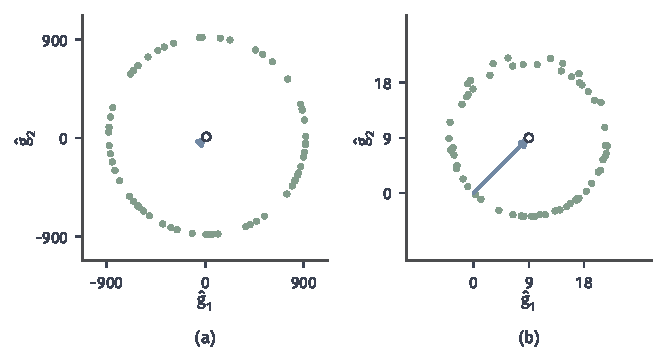
\includegraphics[width=112mm]{figures/05-optimization/05-stochastic-optimization/matplotlib/zo-single-cloud/figure.pdf}
  \caption{贯穿例起点的单点估计，$\delta=0.1$，$60$个随机方向。绿点是估计值，蓝色箭头是真实梯度$(9,9)$，空心圆是它的终点。(a)原读数的估计分布在半径约$900$的圆上，比梯度大两个量级。(b)读数减去常数$45$后，同样的$60$个方向给出的估计缩到半径约$13$的圆上。两张图的坐标范围不同。}
  \label{fig:zo-single-cloud}
\end{BookInlineFigure}

\paragraph{平滑目标的光滑常数}
单点估计常用于$f$只是$G$-Lipschitz的情形。这时$f^{\mathrm{B}}_{\delta}$是否光滑？由恒等式~\eqref{eq:zo-ball-identity}，对任意$\bm{x},\bm{z}$，
\[
 \lVert\nabla f^{\mathrm{B}}_{\delta}(\bm{x})-\nabla f^{\mathrm{B}}_{\delta}(\bm{z})\rVert_2
 \leq\frac{n}{\delta}\mathbb{E}\lvert f(\bm{x}+\delta\bm{u})-f(\bm{z}+\delta\bm{u})\rvert
 \leq\frac{nG}{\delta}\lVert\bm{x}-\bm{z}\rVert_2.
\]
所以$f^{\mathrm{B}}_{\delta}$的光滑常数不超过$nG/\delta$。$\delta$越小，平滑目标越接近原目标，但也越弯曲。这个上界不一定紧，它的作用是说明平滑后有光滑常数可用。

\subsection{双点估计}
\label{sec:zo-two-point}

成对查询允许把单点估计里的大数减掉。在相反方向各读一次，得到\term{双点估计}（two-point estimator）：
\begin{equation}
 \hat{\bm{g}}^{(2)}=\frac{n}{2\delta}\bigl(y_+-y_-\bigr)\bm{u},\qquad
 y_\pm=f(\bm{x}\pm\delta\bm{u}).
 \label{eq:zo-two-point}
\end{equation}
这正是第~\ref{sec:zo-random-direction}节的式~\eqref{eq:zo-random-direction}取$h=\delta$。公式相同，这里的解释却更精确。

\paragraph{为什么均值是平滑梯度}
$\bm{u}$和$-\bm{u}$同分布，所以单点估计用$-\bm{u}$代替$\bm{u}$，期望不变：
\[
 \frac{n}{\delta}\mathbb{E}\bigl[f(\bm{x}+\delta\bm{u})\bm{u}\bigr]
 =\frac{n}{\delta}\mathbb{E}\bigl[f(\bm{x}-\delta\bm{u})(-\bm{u})\bigr].
\]
两式相加除以$2$，右端正是$\mathbb{E}[\hat{\bm{g}}^{(2)}]$，左端由恒等式等于$\nabla f^{\mathrm{B}}_{\delta}(\bm{x})$。于是
\begin{equation}
 \mathbb{E}\bigl[\hat{\bm{g}}^{(2)}\bigr]=\nabla f^{\mathrm{B}}_{\delta}(\bm{x}).
 \label{eq:zo-two-point-mean}
\end{equation}

把两节的说法对照起来，同一个向量有两种读法。作为原梯度的近似，它有偏差，Hessian是Lipschitz时偏差是$O(\delta^2)$；作为平滑梯度的估计，它严格无偏。表~\ref{tab:zo-two-views}列出两种读法的差别。选哪种读法，取决于最终想回答关于哪个目标的问题。

\begin{BookInlineTable}
  \centering
  \begin{tabular}{@{}lll@{}}
    \toprule
    读法 & 估计对象 & 偏差\\
    \midrule
    有限差分 & $\nabla f(\bm{x})$ & 一般非零，随$\delta$缩小\\
    平滑估计 & $\nabla f^{\mathrm{B}}_{\delta}(\bm{x})$ & 严格为零\\
    \bottomrule
  \end{tabular}
  \caption{同一个双点向量的两种读法。原目标不可微时第一种读法没有对象，第二种仍然成立。}
  \label{tab:zo-two-views}
\end{BookInlineTable}

\paragraph{减去中心值的形式}
另一个双点形式把$y_-$换成中心读数：
\begin{equation}
 \hat{\bm{g}}^{(\mathrm{c})}=\frac{n}{\delta}\bigl(f(\bm{x}+\delta\bm{u})-f(\bm{x})\bigr)\bm{u}.
 \label{eq:zo-center-point}
\end{equation}
由$\mathbb{E}[f(\bm{x})\bm{u}]=\bm{0}$，它的均值也是$\nabla f^{\mathrm{B}}_{\delta}(\bm{x})$。两种形式都消除了常数偏移，贯穿例上把“很大的$45$”去掉了。

\paragraph{二阶矩的比较}
消去偏移后，估计的大小由差商决定。下面的引理针对光滑目标给出统一的界。

\begin{lemma}[双点估计的二阶矩]
\label{lem:zo-two-point-moment}
设$\nabla f$是$L$-Lipschitz的，读数精确。对估计~\eqref{eq:zo-two-point}和~\eqref{eq:zo-center-point}，都有
\begin{equation}
 \mathbb{E}\lVert\hat{\bm{g}}\rVert_2^2\leq 2n\lVert\nabla f(\bm{x})\rVert_2^2+\frac{n^2L^2\delta^2}{2}.
 \label{eq:zo-two-point-moment}
\end{equation}
\end{lemma}

\begin{proof}
记$\bm{g}=\nabla f(\bm{x})$，$\hat{\bm{g}}=nD\bm{u}$，其中$D$是对应的差商，写成$D=\langle\bm{g},\bm{u}\rangle+r$。由式~\eqref{eq:zo-central-L}或下降引理，两种形式都有$\lvert r\rvert\leq L\delta/2$。

用$(a+b)^2\leq2a^2+2b^2$和$\lVert\bm{u}\rVert_2=1$，
\[
 \lVert\hat{\bm{g}}\rVert_2^2=n^2D^2\leq 2n^2\langle\bm{g},\bm{u}\rangle^2+\frac{n^2L^2\delta^2}{2}.
\]
取期望，再用$\mathbb{E}[\bm{u}\bm{u}^\top]=\bm{I}/n$，得到结论。
\end{proof}

式~\eqref{eq:zo-two-point-moment}与单点的式~\eqref{eq:zo-one-point-moment}对比，分母里的$\delta^2$不见了，$\delta$可以取得很小而不使估计爆炸。这是精确读数下成对查询的实质收益。

两种双点形式的差别要看函数。贯穿例上，对称形式的差商精确等于方向导数，二阶矩是$n\lVert\bm{g}\rVert_2^2$；中心形式多出$\tfrac{\delta}{2}\bm{u}^\top\bm{H}\bm{u}$，二阶矩更大。在极小点$\bm{g}=\bm{0}$处，对称形式的估计恒为零，而中心形式不为零，这点上对称形式完全不抖动。$f=\lvert x\rvert$在$x=0$处，对称形式同样恒为零，中心形式的估计是$\pm1$。

但是“方差改善”不是无条件的结论。第一，改善来自消去$f$的大小，如果$f$本身在零附近，单点估计并没有这部分额外的方差。第二，带独立噪声时，两次单点估计取平均与一次双点估计噪声贡献相同，都是$n^2\sigma^2/(2\delta^2)$，第~\ref{sec:zo-pair-noise}节会算出来。所以成对读数消去的是函数值的公共部分，不是噪声。

\subsection{高斯方向估计}
\label{sec:zo-gaussian}

球面方向需要扰动恰好落在半径$\delta$的球面上。如果改用高斯扰动，查询点不再被限制在球面上，分析也更简单，因为高斯密度的导数有封闭形式。

\paragraph{主要思想}
作变量替换$\bm{z}=\bm{x}+\tau\bm{w}$，把高斯平滑写成
\[
 f^{\mathrm{G}}_{\tau}(\bm{x})=\frac{1}{(2\pi\tau^2)^{n/2}}\int f(\bm{z})\exp\Bigl(-\frac{\lVert\bm{z}-\bm{x}\rVert_2^2}{2\tau^2}\Bigr)\mathrm{d}\bm{z}.
\]
现在$\bm{x}$只出现在指数里，$f$不必可微，梯度全部落到光滑的高斯核上。这与球平滑的情况类似：导数从$f$转移到了平均方式上。

\begin{theorem}[高斯平滑的梯度恒等式]
\label{thm:zo-gauss-identity}
设$f$可测，存在$C,a\geq0$使$\lvert f(\bm{z})\rvert$处处不超过$Ce^{a\lVert\bm{z}\rVert_2}$，$\bm{w}\sim\mathcal{N}(\bm{0},\bm{I})$。则$f^{\mathrm{G}}_{\tau}$可微，且
\begin{equation}
 \nabla f^{\mathrm{G}}_{\tau}(\bm{x})=\frac{1}{\tau}\,\mathbb{E}_{\bm{w}}\bigl[f(\bm{x}+\tau\bm{w})\,\bm{w}\bigr].
 \label{eq:zo-gauss-identity}
\end{equation}
\end{theorem}

\begin{proof}
高斯核对$\bm{x}$的梯度等于核本身乘$(\bm{z}-\bm{x})/\tau^2$。当$\bm{x}$在一个有界邻域内时，被积函数对$\bm{x}$的梯度被一个不依赖$\bm{x}$的可积函数控制：指数增长被高斯衰减压住。由控制收敛定理，可在积分号下求导，得
\[
 \nabla f^{\mathrm{G}}_{\tau}(\bm{x})=\frac{1}{(2\pi\tau^2)^{n/2}}\int f(\bm{z})\frac{\bm{z}-\bm{x}}{\tau^2}\exp\Bigl(-\frac{\lVert\bm{z}-\bm{x}\rVert_2^2}{2\tau^2}\Bigr)\mathrm{d}\bm{z}.
\]
再换回$\bm{z}=\bm{x}+\tau\bm{w}$，$(\bm{z}-\bm{x})/\tau^2=\bm{w}/\tau$，即得结论。
\end{proof}

这个定理比球面的恒等式要求的局部性质弱：$f$可以不连续，因为积分覆盖整个空间，$f$在零测集上的值不起作用。要求转移到了全局的增长上，这正好是定义中高斯平滑存在所需要的。

\paragraph{三种形式}
抽一个$\bm{w}$，式~\eqref{eq:zo-gauss-identity}给出单点形式。与球面的情形一样，减去中心值或取对称差，均值不变：
\begin{equation}
 \hat{\bm{g}}^{\mathrm{G}}=\frac{y}{\tau}\bm{w},\qquad
 \hat{\bm{g}}^{\mathrm{Gc}}=\frac{y-f(\bm{x})}{\tau}\bm{w},\qquad
 \hat{\bm{g}}^{\mathrm{Gs}}=\frac{y-y'}{2\tau}\bm{w},
 \label{eq:zo-gauss-estimators}
\end{equation}
其中$y=f(\bm{x}+\tau\bm{w})$，$y'=f(\bm{x}-\tau\bm{w})$。第二种利用了$\mathbb{E}[\bm{w}]=\bm{0}$，第三种利用了$\bm{w}$与$-\bm{w}$同分布。

贯穿例起点，取$\tau=0.1$，抽到$\bm{w}=(1,-0.5)$。对称形式的读数和差商是
\[
 f(9.1,0.95)=45.46625,\qquad f(8.9,1.05)=44.56625,\qquad\frac{y-y'}{2\tau}=4.5.
\]
这里$\langle\nabla f,\bm{w}\rangle=9-4.5=4.5$，吻合。估计是$4.5\,\bm{w}=(4.5,-2.25)$。

\paragraph{与球面方向的区别}
公式里没有因子$n$，这是因为$\mathbb{E}[\bm{w}\bm{w}^\top]=\bm{I}$，球面方向则是$\bm{I}/n$。如果把球面的归一化照搬过来写成$(n/\tau)y\bm{w}$，二次函数上的均值就变成$n\nabla f$，整整放大$n$倍。

另一个区别是扰动的长度。$\lVert\bm{w}\rVert_2$是随机的，大约是$\sqrt{n}$，如图~\ref{fig:zo-sphere-gauss}(b)。$\tau$只是尺度，不是查询半径。$n=2$时
\[
 \mathbb{P}\bigl(\lVert\bm{w}\rVert_2>3\bigr)=e^{-4.5}\approx0.011,
\]
一百次里约有一次偏离三个尺度。要与球面半径$\delta$对应，应取$\tau=\delta/\sqrt{n}$，这时$\tau\bm{w}$的均方长度等于$\delta^2$。

\begin{BookInlineFigure}
  \centering
  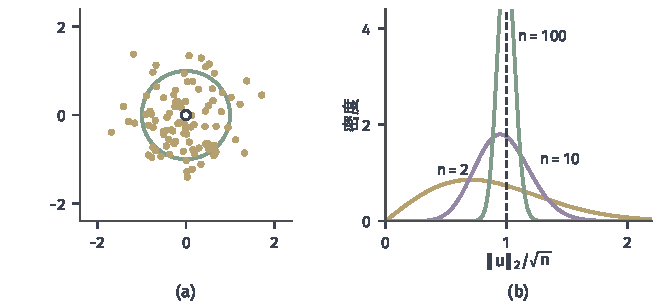
\includegraphics[width=112mm]{figures/05-optimization/05-stochastic-optimization/matplotlib/zo-sphere-gauss/figure.pdf}
  \caption{球面方向与高斯方向。(a)$n=2$，绿圆是半径$\delta=1$的球面查询位置，黄点是尺度$\tau=1/\sqrt{2}$的高斯查询点，二者均方长度相同，高斯点散布在圆内外。(b)$\lVert\bm{w}\rVert_2/\sqrt{n}$的密度。维数增大时高斯方向的长度集中到$\sqrt{n}$附近，$n=2$时差异很大。}
  \label{fig:zo-sphere-gauss}
\end{BookInlineFigure}

二次函数上，对称形式的二阶矩可以直接算：
\[
 \mathbb{E}\bigl[\langle\bm{g},\bm{w}\rangle^2\lVert\bm{w}\rVert_2^2\bigr]=(n+2)\lVert\bm{g}\rVert_2^2.
\]
所以方差是$(n+1)\lVert\bm{g}\rVert_2^2$，比球面方向的$(n-1)\lVert\bm{g}\rVert_2^2$略大，多出来的部分来自长度的波动。一般光滑函数上有类似的上界：
\begin{equation}
 \mathbb{E}\lVert\hat{\bm{g}}^{\mathrm{Gs}}\rVert_2^2\leq2(n+2)\lVert\nabla f(\bm{x})\rVert_2^2+\frac{L^2\tau^2}{2}n(n+2)(n+4).
 \label{eq:zo-gauss-moment}
\end{equation}
推导与引理~\ref{lem:zo-two-point-moment}相同，只是余项是$\lvert r\rvert\leq L\tau\lVert\bm{w}\rVert_2^2/2$，再用高斯矩$\mathbb{E}\lVert\bm{w}\rVert_2^6=n(n+2)(n+4)$。

\subsection{成对读数的噪声}
\label{sec:zo-pair-noise}

到此为止的二阶矩都假设读数精确。本小节回到第~\ref{sec:zo-pair-interface}节的接口问题：读数含噪声时，成对差分的波动是多少？

\paragraph{独立噪声}
采用式~\eqref{eq:zo-independent-pair}，$\zeta_+,\zeta_-$条件独立，均值零，方差不超过$\sigma^2$。差商的噪声部分是$(\zeta_+-\zeta_-)/(2\delta)$，于是
\begin{equation}
 \operatorname{Var}\Bigl(\frac{\zeta_+-\zeta_-}{2\delta}\Bigr)\leq\frac{\sigma^2}{2\delta^2}.
 \label{eq:zo-independent-variance}
\end{equation}
半径减半，方差变成四倍。噪声大小不随距离变小，分母却在变小。图~\ref{fig:zo-pair-noise}中黄线的斜率是$-2$。

噪声与差商主项的交叉项为零，因为噪声的条件均值是零。代入估计，$\lVert\hat{\bm{g}}^{(2)}\rVert_2^2$的期望增加$n^2\sigma^2/(2\delta^2)$。结合引理~\ref{lem:zo-two-point-moment}，得到后面反复使用的二阶矩界：
\begin{equation}
 \mathbb{E}\lVert\hat{\bm{g}}^{(2)}\rVert_2^2\leq2n\lVert\nabla f(\bm{x})\rVert_2^2+V,\qquad
 V=\frac{n^2L^2\delta^2}{2}+\frac{n^2\sigma^2}{2\delta^2}.
 \label{eq:zo-noisy-moment}
\end{equation}

\paragraph{单点平均与成对差分}
单点估计用两次独立读数和两个独立方向取平均时，噪声贡献是
\[
 \frac14\Bigl(\frac{n^2\sigma^2}{\delta^2}+\frac{n^2\sigma^2}{\delta^2}\Bigr)=\frac{n^2\sigma^2}{2\delta^2},
\]
与双点估计完全相同。这验证了前面的说法：独立噪声下，配对不减少噪声，只消去函数值的公共部分。

\paragraph{共享样本}
采用式~\eqref{eq:zo-shared-pair}，差分的方差包含协方差：
\begin{equation}
 \operatorname{Var}\bigl[F(\bm{q}_+;\bm{\xi})-F(\bm{q}_-;\bm{\xi})\bigr]
 =\operatorname{Var}F_++\operatorname{Var}F_--2\operatorname{Cov}(F_+,F_-).
 \label{eq:zo-shared-variance}
\end{equation}
共享样本带来的是正的协方差，协方差越大，抵消越多。若两个噪声的相关系数是$\rho$且方差都是$\sigma^2$，差的方差是$2\sigma^2(1-\rho)$，从$\rho=0$的独立到$\rho=1$的完全抵消，中间是连续变化的。

\paragraph{三个例子}
共享样本的效果取决于样本函数本身的波动。

第一个例子是两点共享同一个加性噪声，$F(\bm{x};\xi)=f(\bm{x})+\xi$。差分时$\xi$完全消失，噪声方差为零，无论半径多小，差商都是精确的。

第二个例子是样本函数关于$\bm{x}$Lipschitz，比如$F(\bm{x};\bm{\xi})=f(\bm{x})+\bm{\xi}^\top\bm{x}$。差分的随机部分是
\[
 \frac{\bm{\xi}^\top(\bm{q}_+-\bm{q}_-)}{2\delta}=\bm{\xi}^\top\bm{u},
\]
它不依赖$\delta$。一般地，若$F(\cdot;\bm{\xi})$是Lipschitz的，常数为$G(\bm{\xi})$，差商的二阶矩不超过$\mathbb{E}[G(\bm{\xi})^2]$，$\delta$可以取得很小。图~\ref{fig:zo-pair-noise}中绿线是水平的。

第三个例子是样本函数不连续。$F(x;\xi)=\mathbb{1}\{x>\xi\}$，$\xi$的密度为$p$。共享$\xi$时差分只在$\xi\in[x-h,x+h)$时非零，概率约$2hp(x)$，于是差商方差约为
\[
 \frac{2hp(x)}{4h^2}=\frac{p(x)}{2h}.
\]
它比独立噪声的$1/h^2$好，但仍随$h$缩小而增大，图~\ref{fig:zo-pair-noise}中紫线的斜率是$-1$。所以共享样本带来改善的前提是差值的波动受控，只说“用了同一个种子”并不够。

\begin{BookInlineFigure}
  \centering
  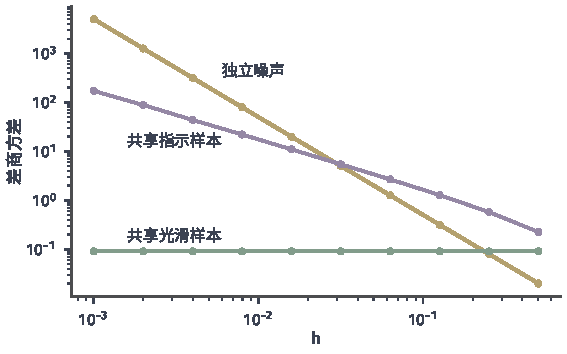
\includegraphics[width=96mm]{figures/05-optimization/05-stochastic-optimization/matplotlib/zo-pair-noise/figure.pdf}
  \caption{中心差商的方差随$h$的变化，$x=0.5$。黄线：独立加性噪声，标准差$0.1$，斜率$-2$。紫线：共享指示样本$F=\mathbb{1}\{x>\xi\}$，$\xi\sim\mathcal{N}(0,1)$，斜率$-1$。绿线：共享光滑样本$F=x^2/2+\xi x$，$\xi$标准差$0.3$，方差不随$h$变化。共享同一加性噪声时方差为零，未画出。每点来自$4\times10^6$次模拟。}
  \label{fig:zo-pair-noise}
\end{BookInlineFigure}

\section{零阶随机梯度方法}
\label{sec:zo-method}

前两节构造了各种方向估计。接下来要弄清：把它们放进迭代后，算法实际在优化什么，步长和扰动尺度怎样定，遇到约束怎么办，最后交出什么结果？

\subsection{基本迭代}
\label{sec:zo-basic}

\paragraph{主要思想}
第~\ref{chap:stochastic-gradient-methods}章的随机更新沿随机方向$\hat{\bm{g}}^{(t)}$的负向走一步。它能用的原因是，这个方向平均起来指向某个函数的梯度。零阶方法沿用这个更新，只是$\hat{\bm{g}}^{(t)}$由函数值算出：
\begin{equation}
 \bm{x}^{(t+1)}=\bm{x}^{(t)}-\alpha^{(t)}\hat{\bm{g}}^{(t)},\qquad
 \hat{\bm{g}}^{(t)}=\frac{n}{2\delta}\bigl(y_+^{(t)}-y_-^{(t)}\bigr)\bm{u}^{(t)}.
 \label{eq:zo-update}
\end{equation}
这是\term{零阶随机梯度方法}（zeroth-order stochastic gradient method）的双点形式，其他估计器可以替换第二式。一轮的流程如图~\ref{fig:zo-flow}所示。

\begin{BookInlineFigure}
  \centering
  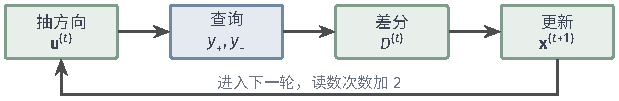
\includegraphics[width=105mm]{figures/05-optimization/05-stochastic-optimization/tikz/zo-flow/figure.pdf}
  \caption{双点零阶方法的一轮。绿框是算法内部的计算，蓝框是向黑箱提交的查询。每轮两次函数读数，查询预算按读数次数累计。}
  \label{fig:zo-flow}
\end{BookInlineFigure}

更新形式都一样，算法朝哪里走却由估计器的条件均值决定，不能只看形式。式~\eqref{eq:zo-update}的条件均值是$\nabla f^{\mathrm{B}}_{\delta}(\bm{x}^{(t)})$，所以它是平滑目标上的随机梯度方法，不是原目标上的。

\needspace{6\baselineskip}
\paragraph{变量}
\begin{itemize}
 \item $\bm{x}^{(t)}\in\mathbb{R}^n$：当前迭代点。
 \item $\bm{u}^{(t)}\in\bm{S}$：本轮的单位方向，$n$维。
 \item $y_\pm^{(t)}$：两次读数，标量。
 \item $D^{(t)}=(y_+^{(t)}-y_-^{(t)})/(2\delta)$：差商，标量。
 \item $\hat{\bm{g}}^{(t)}\in\mathbb{R}^n$：方向估计。
 \item $\alpha$、$\delta$：步长与扰动半径，取常数。
 \item $Q$：已用读数次数。
\end{itemize}

\paragraph{初始化}
取起点$\bm{x}^{(0)}$，选定$\alpha$、$\delta$和读数预算$Q_{\max}$，令$Q=0$。例中目标是贯穿例~\eqref{eq:zo-example}，读数带独立噪声，并取
\[
 \bm{x}^{(0)}=(9,1),\quad\alpha=0.05,\quad\delta=0.5,\quad Q_{\max}=6.
\]

\needspace{6\baselineskip}
\paragraph{每轮更新}
下面的数值用事先给定的方向和噪声，便于逐项核对。
\begin{enumerate}
 \item 抽取方向$\bm{u}^{(t)}$。例中第一轮$\bm{u}^{(0)}=(0.6,0.8)$，第二轮$\bm{u}^{(1)}=(0.8,-0.6)$，第三轮$\bm{u}^{(2)}=(0.28,0.96)$。
 \item 查询$\bm{x}^{(t)}\pm\delta\bm{u}^{(t)}$，$Q$增加$2$。例中第一轮两个查询点是$(9.3,1.4)$和$(8.7,0.6)$，真实函数值为$52.065$和$39.465$，噪声分别为$+0.1$和$-0.1$，读数是
 \[
  y_+^{(0)}=52.165,\qquad y_-^{(0)}=39.365.
 \]
 \item 由式~\eqref{eq:zo-update}算差商和方向估计。例中$2\delta=1$，$n=2$，第一轮结果是
 \[
  D^{(0)}=12.8,\qquad\hat{\bm{g}}^{(0)}=2\cdot12.8\cdot(0.6,0.8)=(15.36,\ 20.48).
 \]
 \item 由式~\eqref{eq:zo-update}沿$-\hat{\bm{g}}^{(t)}$走步长$\alpha$。例中第一轮得到
 \[
  \bm{x}^{(1)}=(9,1)-0.05\,(15.36,20.48)=(8.232,\ -0.024).
 \]
\end{enumerate}

第二轮从$\bm{x}^{(1)}$出发，查询点是$(8.632,-0.324)$和$(7.832,0.276)$，噪声是$-0.1$和$+0.1$，读数和结果为
\[
 y_+^{(1)}\approx37.628,\quad y_-^{(1)}\approx31.113,\quad D^{(1)}\approx6.515,
\]
\[
 \hat{\bm{g}}^{(1)}\approx(10.424,\ -7.818),\qquad\bm{x}^{(2)}\approx(7.711,\ 0.367).
\]

第三轮查询点是$(7.851,0.847)$和$(7.571,-0.113)$，噪声是$+0.05$和$+0.15$，读数和结果为
\[
 y_+^{(2)}\approx34.095,\quad y_-^{(2)}\approx28.866,\quad D^{(2)}\approx5.229,
\]
\[
 \hat{\bm{g}}^{(2)}\approx(2.928,\ 10.040),\qquad\bm{x}^{(3)}\approx(7.564,\ -0.135).
\]

迭代在$Q$达到$Q_{\max}$时结束。例中三轮用完$6$次读数，最终得到$\bm{x}^{(3)}\approx(7.564,-0.135)$，真实目标值约$28.69$，从$45$下降了三分之一多。第二轮的梯度第二分量只有$-0.216$，估计的第二分量却是$-7.818$，$x_2$从$-0.024$跳到$0.367$，这种摆动是单方向估计的常态。继续运行的结果见图~\ref{fig:zo-paths}。

\begin{BookInlineFigure}
  \centering
  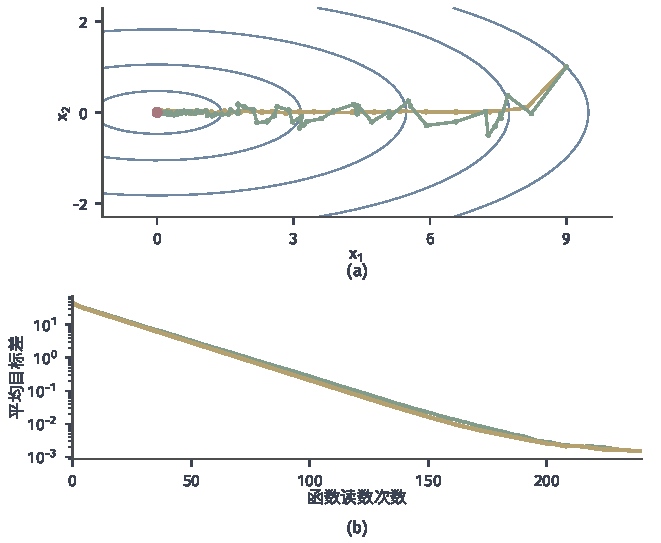
\includegraphics[width=112mm]{figures/05-optimization/05-stochastic-optimization/matplotlib/zo-paths/figure.pdf}
  \caption{贯穿例上的零阶迭代，读数噪声标准差$0.1$。(a)绿线是双点球面方法的一次运行，$\alpha=0.05$，$\delta=0.5$，前三轮即正文手算的数据，共$120$轮；黄线是中心坐标差分的梯度下降，$\alpha=0.1$，$h=0.5$，共$60$轮；蓝线是等高线，红点是解。(b)$200$次运行的平均目标差，横轴是函数读数次数。}
  \label{fig:zo-paths}
\end{BookInlineFigure}

图~\ref{fig:zo-paths}(a)中绿线抖动，黄线平稳，但按读数次数算两者几乎重合，如图~\ref{fig:zo-paths}(b)。这里两者的步长不同：单方向估计的步长要比完整梯度小一个与$n$相关的倍数，原因在第~\ref{sec:zo-step-scale}节说明。

\paragraph{多方向平均}
每轮抽$m$个独立方向，分别计算估计后取平均，是最常见的变体，一轮用$2m$次读数：
\begin{equation}
 \hat{\bm{g}}^{(t)}=\frac{1}{m}\sum_{j=1}^{m}\frac{n}{2\delta}\bigl(y_{j,+}^{(t)}-y_{j,-}^{(t)}\bigr)\bm{u}_j^{(t)}.
 \label{eq:zo-multi-direction}
\end{equation}
条件均值不变，方差变成$1/m$。例中第一轮若用$\bm{u}_1=(0.6,0.8)$和$\bm{u}_2=(0.8,-0.6)$两个方向，不计噪声时，两个估计是
\[
 (15.12,\ 20.16),\qquad(2.88,\ -2.16).
\]
它们的平均恰为$(9,9)$，这时$\bm{x}^{(1)}=(8.55,0.55)$。两个方向正交且数量等于维数，对二次函数恰好拼出了完整梯度。

\paragraph{一步分析：有偏与无偏两条路}
把估计器代入迭代，有两种分析方式，对应前面的两种读法。先假设$\nabla f$是$L$-Lipschitz的，第一种直接看原目标。

\begin{lemma}[单步下降]
\label{lem:zo-one-step}
设$\bm{x}^+=\bm{x}-\alpha\hat{\bm{g}}$，$\nabla f$是$L$-Lipschitz的。若$\hat{\bm{g}}$的条件均值是$\nabla f(\bm{x})+\bm{b}$，且$\lVert\bm{b}\rVert_2\leq\beta$，则
\begin{equation}
 \mathbb{E}[f(\bm{x}^+)\mid\bm{x}]\leq f(\bm{x})-\frac{\alpha}{2}\lVert\nabla f(\bm{x})\rVert_2^2+\frac{\alpha}{2}\beta^2+\frac{L\alpha^2}{2}\mathbb{E}\bigl[\lVert\hat{\bm{g}}\rVert_2^2\mid\bm{x}\bigr].
 \label{eq:zo-biased-step}
\end{equation}
若$\hat{\bm{g}}$的条件均值是$\nabla f^{\mathrm{B}}_{\delta}(\bm{x})$，则
\begin{equation}
 \mathbb{E}[f^{\mathrm{B}}_{\delta}(\bm{x}^+)\mid\bm{x}]\leq f^{\mathrm{B}}_{\delta}(\bm{x})-\alpha\lVert\nabla f^{\mathrm{B}}_{\delta}(\bm{x})\rVert_2^2+\frac{L\alpha^2}{2}\mathbb{E}\bigl[\lVert\hat{\bm{g}}\rVert_2^2\mid\bm{x}\bigr].
 \label{eq:zo-unbiased-step}
\end{equation}
\end{lemma}

\begin{proof}
由下降引理，对$L$-光滑函数$\psi$，
\[
 \psi(\bm{x}^+)\leq\psi(\bm{x})-\alpha\langle\nabla\psi(\bm{x}),\hat{\bm{g}}\rangle+\frac{L\alpha^2}{2}\lVert\hat{\bm{g}}\rVert_2^2.
\]
取$\psi=f$并取条件期望，内积项变为$-\alpha\lVert\nabla f\rVert_2^2-\alpha\langle\nabla f,\bm{b}\rangle$。再用
\[
 -\langle\nabla f,\bm{b}\rangle\leq\frac12\lVert\nabla f\rVert_2^2+\frac12\beta^2,
\]
得式~\eqref{eq:zo-biased-step}。

取$\psi=f^{\mathrm{B}}_{\delta}$，由引理~\ref{lem:zo-smoothing-properties}，它也是$L$-光滑的，内积项的条件期望是$-\alpha\lVert\nabla f^{\mathrm{B}}_{\delta}\rVert_2^2$，得式~\eqref{eq:zo-unbiased-step}。
\end{proof}

两式对比可以看出两种分析的差别。式~\eqref{eq:zo-biased-step}留下了偏差项$\tfrac{\alpha}{2}\beta^2$，它每步都存在，累加后构成不会随步数消失的误差。式~\eqref{eq:zo-unbiased-step}没有偏差项，账记在平滑目标上，代价是结论说的是$f^{\mathrm{B}}_{\delta}$，要回到$f$还须另算，这留给第~\ref{sec:zo-original-error}节。

\subsection{步长与扰动尺度}
\label{sec:zo-step-scale}

这里有两个旋钮。步长$\alpha$决定参数实际走多远，扰动尺度$\delta$决定在多大的邻域里比较函数值。两者的量纲都不同：改变$\delta$不移动$\bm{x}$，只改变估计的性质。

\paragraph{步长的上限}
由式~\eqref{eq:zo-noisy-moment}，二阶矩中有$2n\lVert\nabla f\rVert_2^2$，比完整梯度的$\lVert\nabla f\rVert_2^2$大$2n$倍。代入式~\eqref{eq:zo-unbiased-step}，要让下降项压住二阶矩项，需要$\alpha\lesssim1/(nL)$。直观地说，估计的长度波动约为梯度的$\sqrt{n}$倍，步长必须相应地收小。

这个步长要与每轮的读数次数放在一起看。完整坐标差分的步长是$1/L$，但每轮要$2n$次读数；单方向的步长是$1/(nL)$，每轮$2$次读数。按读数次数算，两者每次读数的“进展”同阶，这就是图~\ref{fig:zo-paths}(b)中两条曲线重合的原因。

贯穿例的手算用了$\alpha=0.05<1/(nL)=1/18$。下一小节定理要求的$\alpha\leq1/(4nL)=1/72$更保守，这是为了在任意光滑函数上保证下降，实际使用时常可放宽。

\paragraph{固定尺度对应固定的平滑目标}
$\delta$固定时，迭代是同一个$f^{\mathrm{B}}_{\delta}$上的随机梯度方法，所以固定步长最终会停在一个噪声水平上。图~\ref{fig:zo-delta-floor}(a)在贯穿例上取$\alpha=0.02$，噪声$\sigma=1$，分别用$\delta=0.1,0.5,2$。

三条曲线下降段相同，稳定后的水平差别很大，$\delta$从$0.1$增大到$0.5$，水平约下降$25$倍。这正是式~\eqref{eq:zo-noisy-moment}中$V$的噪声项$n^2\sigma^2/(2\delta^2)$的$1/\delta^2$规律。这个例子是二次函数，平滑没有引入任何偏差，所以$\delta$越大越好；一般函数上$\delta$还有偏差的代价，第~\ref{sec:zo-tradeoff}节讨论。

\begin{BookInlineFigure}
  \centering
  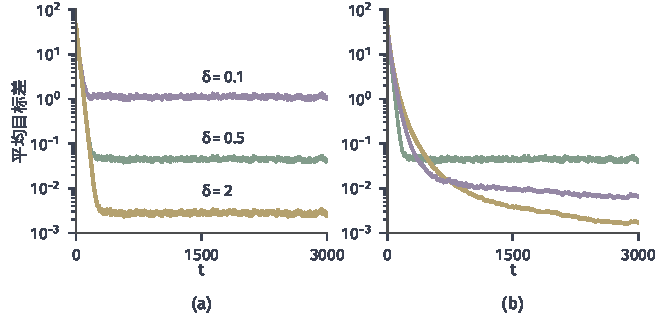
\includegraphics[width=112mm]{figures/05-optimization/05-stochastic-optimization/matplotlib/zo-delta-floor/figure.pdf}
  \caption{贯穿例上双点方法的平均目标差，读数噪声$\sigma=1$，$300$次运行。(a)固定$\alpha=0.02$，紫、绿、黄三线分别为$\delta=0.1,0.5,2$，稳定水平按$1/\delta^2$变化。(b)$\delta=0.5$时固定$\alpha=0.02$（绿）；步长递减$\alpha^{(t)}=0.02/(1+t/100)$（黄）；步长递减较慢、尺度也递减，$\alpha^{(t)}=0.02/(1+t/100)^{0.75}$，$\delta^{(t)}=0.5/(1+t/100)^{0.1}$（紫）。}
  \label{fig:zo-delta-floor}
\end{BookInlineFigure}

\paragraph{递减步长}
要越过这个水平，步长必须递减，这与第~\ref{chap:stochastic-gradient-methods}章的情形相同。图~\ref{fig:zo-delta-floor}(b)的黄线就是在$\delta$固定时让步长递减，曲线继续下降。

\paragraph{逐步缩小尺度要多记两笔}
既然小的$\delta$偏差小，能否让$\delta^{(t)}$随迭代缩小？可以，但目标函数本身在变，分析要多记两笔。

第一笔是目标的变化。第$t$步看的是$f^{\mathrm{B}}_{\delta^{(t)}}$，下一步换成$f^{\mathrm{B}}_{\delta^{(t+1)}}$，累加时不再是同一个函数相减，多出差值$f^{\mathrm{B}}_{\delta^{(t+1)}}-f^{\mathrm{B}}_{\delta^{(t)}}$。若$\delta^{(t+1)}\leq\delta^{(t)}$，由式~\eqref{eq:zo-ball-error}，这个差值的绝对值不超过$L(\delta^{(t)})^2$，一般情形要把它们加起来，$\sum_t(\delta^{(t)})^2$必须受控。

凸函数的情形方便一些。设$\delta_1\leq\delta_2$，$\lambda=\delta_1/\delta_2$。由凸性，
\[
 f(\bm{x}+\delta_1\bm{v})\leq\lambda f(\bm{x}+\delta_2\bm{v})+(1-\lambda)f(\bm{x}).
\]
取期望并用$f\leq f^{\mathrm{B}}_{\delta_2}$，得
\[
 f^{\mathrm{B}}_{\delta_1}\leq f^{\mathrm{B}}_{\delta_2}.
\]
所以缩小半径时平滑目标只降不升，这一笔差值对凸函数不造成损失。

第二笔是方差的变化。$V$里的噪声项是$n^2\sigma^2/(2(\delta^{(t)})^2)$，缩小$\delta$会放大方差，步长必须缩得更快，抵消这部分增长。累加式~\eqref{eq:zo-unbiased-step}可见需要控制的是$\sum_t(\alpha^{(t)})^2V^{(t)}$，因此独立噪声下的标准要求是
\begin{equation}
 \sum_t\alpha^{(t)}=\infty,\qquad
 \sum_t\Bigl(\frac{\alpha^{(t)}}{\delta^{(t)}}\Bigr)^2<\infty,\qquad
 \delta^{(t)}\to0.
 \label{eq:zo-schedule}
\end{equation}
前一个条件保证能走得足够远，后一个条件是随机逼近步长条件的变形\scite{math-robbins1951stochastic}，分母上多了$\delta^{(t)}$，反映差商的噪声放大。图~\ref{fig:zo-delta-floor}(b)的紫线步长递减更慢，尺度也在缩小，两者都使噪声项更大，所以高于黄线。这个二次函数上$\delta$没有偏差可减，缩小尺度没有收益，这也说明$\delta$是否该缩小要看偏差。

\subsection{约束下的查询}
\label{sec:zo-constrained-query}

约束问题要多考虑一件事：不光更新点要可行，查询点也可能需要可行。仿真器在非法参数下可能崩溃，物理实验在限制之外可能损坏设备。

\paragraph{更新可行不等于查询可行}
投影更新
\[
 \bm{x}^{(t+1)}=\Pi_{\bm{C}}\bigl(\bm{x}^{(t)}-\alpha\hat{\bm{g}}^{(t)}\bigr)
\]
保证了迭代点在$\bm{C}$内，但没有限制查询点。以$\bm{C}=[1,9]\times[-1,1]$为例，$\bm{x}=(1,0.4)$在边界上，取$\delta=0.2$，$\bm{u}=(0.6,0.8)$，两个查询点是
\[
 \bm{x}+\delta\bm{u}=(1.12,\ 0.56),\qquad\bm{x}-\delta\bm{u}=(0.88,\ 0.24).
\]
第二个点的$x_1<1$，越出了可行域，如图~\ref{fig:zo-constrained}(a)。投影把迭代点拉回来，却管不到这一步。

\begin{BookInlineFigure}
  \centering
  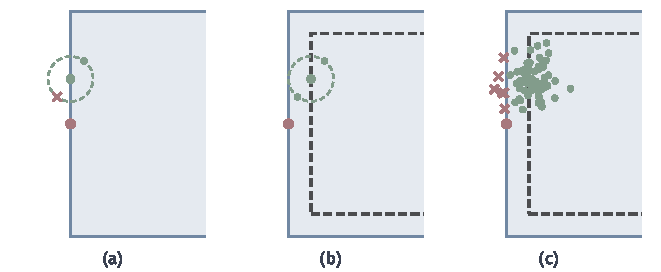
\includegraphics[width=112mm]{figures/05-optimization/05-stochastic-optimization/matplotlib/zo-constrained/figure.pdf}
  \caption{可行域$\bm{C}=[1,9]\times[-1,1]$的左端（浅蓝），红点是贯穿例在$\bm{C}$上的解$(1,0)$，绿点是迭代点和可行的查询点，红叉是越界查询。(a)迭代点在边界上，半径$0.2$的查询圆（绿色虚线）越界，$(0.88,0.24)$不可行。(b)把迭代点限制在内缩域（灰色虚线），查询圆完全在$\bm{C}$内。(c)同样的内缩域，尺度$\tau=\delta/\sqrt{2}$的高斯扰动仍有查询点越界。}
  \label{fig:zo-constrained}
\end{BookInlineFigure}

\paragraph{收缩查询区域}
解决办法是把迭代点限制在一个内缩的区域里，让半径$\delta$的球放得下。设凸集$\bm{C}$含有以原点为心、半径$r$的球，即$r\bm{B}\subseteq\bm{C}$。令$\theta=\delta/r\in(0,1)$，取收缩集合
\begin{equation}
 \bm{C}_\theta=(1-\theta)\bm{C}.
 \label{eq:zo-shrink}
\end{equation}

\begin{theorem}[收缩集合的查询可行性与边界误差]
\label{thm:zo-shrink}
设$\bm{C}$是凸集，$r\bm{B}\subseteq\bm{C}$，$\theta=\delta/r<1$。则对$\bm{x}\in\bm{C}_\theta$和$\bm{v}\in\bm{B}$，有$\bm{x}+\delta\bm{v}\in\bm{C}$。若$f$在$\bm{C}$上是凸函数，$\bm{x}^\star\in\bm{C}$是解，则
\begin{equation}
 \min_{\bm{x}\in\bm{C}_\theta}f(\bm{x})-f^\star\leq\theta\bigl(f(\bm{0})-f^\star\bigr).
 \label{eq:zo-shrink-error}
\end{equation}
\end{theorem}

\begin{proof}
设$\bm{x}=(1-\theta)\bm{c}$，$\bm{c}\in\bm{C}$。则
\[
 \bm{x}+\delta\bm{v}=(1-\theta)\bm{c}+\theta\,(r\bm{v}),
\]
这里用了$\delta=\theta r$。右端是$\bm{C}$中两点$\bm{c}$和$r\bm{v}$的凸组合，所以在$\bm{C}$中。

误差界：$(1-\theta)\bm{x}^\star\in\bm{C}_\theta$，由凸性，
\[
 f\bigl((1-\theta)\bm{x}^\star+\theta\bm{0}\bigr)\leq(1-\theta)f^\star+\theta f(\bm{0}).
\]
移项即得。
\end{proof}

定理的条件中，内部球不可少：$r$越小，同样的$\delta$需要收缩得越多，$\bm{C}$没有内点时完全无法在$\bm{C}$内做全维扰动。凸性用在了两处，凸组合的可行性和最后的误差界。

继续上面的例子，以$(5,0)$为中心平移，$\bm{C}$含半径$r=1$的球。$\delta=0.2$时$\theta=0.2$，$\bm{C}_\theta=[1.8,8.2]\times[-0.8,0.8]$。解$(1,0)$被挡在外面，$\bm{C}_\theta$上最好的点是$(1.8,0)$，代价是$f(1.8,0)-f(1,0)=1.12$，定理的上界是$0.2\cdot(12.5-0.5)=2.4$。按比例收缩对长边很不划算。

如果知道$\bm{C}$的形状，直接用内缩集$\{\bm{x}:\bm{x}+\delta\bm{B}\subseteq\bm{C}\}$更好。这里它是$[1.2,8.8]\times[-0.8,0.8]$，如图~\ref{fig:zo-constrained}(b)，代价只有$f(1.2,0)-f(1,0)=0.22$。

收缩产生的误差要计入最终结果：算法解的是$\bm{C}_\theta$上的问题，$\delta$越大这笔误差越大，同时噪声方差越小，这是约束情形下多出来的一层取舍。

\paragraph{高斯扰动的问题}
高斯分布的支撑是全空间，从任何一点出发都有正概率越界，如图~\ref{fig:zo-constrained}(c)，收缩多少都无法消除。要用高斯扰动，必须有办法在域外查询：比如$f$有明确的域外延拓，且恒等式~\eqref{eq:zo-gauss-identity}所需的增长条件在延拓后成立，那么平滑目标就是延拓函数的平滑。

如果域外不能查询，把越界的点投影回来或截断分布都会改变查询点的分布，恒等式不再成立，需要另行设计估计器并重新分析它的偏差。

\subsection{输出与停止}
\label{sec:zo-output}

迭代结束时要交出一个点，并且说明它满足什么保证。下面先给无约束情形的两个基本结论，它们的累加方式与一阶方法相同，只是二阶矩换成了零阶估计的二阶矩。

\paragraph{光滑非凸情形}
非凸目标上只能期望梯度变小。迭代序列上最小的梯度无法用读数辨认，所以常用随机返回：事先在$\{0,\ldots,T-1\}$上均匀抽取下标$R$，输出$\bm{x}^{(R)}$\scite{ghadimi2013stochastic}。这样输出点的期望恰好等于全部迭代的平均。

\begin{theorem}[光滑非凸目标]
\label{thm:zo-nonconvex}
设$\nabla f$是$L$-Lipschitz的，$f\geq f_{\inf}$，读数带独立噪声，方差不超过$\sigma^2$（$\sigma=0$为精确读数）。迭代~\eqref{eq:zo-update}取常数$\alpha\leq1/(4nL)$，常数$\delta>0$。记
\begin{equation}
 \Delta_\delta=f^{\mathrm{B}}_{\delta}(\bm{x}^{(0)})-f_{\inf},\qquad W=4nL^2\delta^2+V,
 \label{eq:zo-nonconvex-constants}
\end{equation}
其中$V$见式~\eqref{eq:zo-noisy-moment}。则
\begin{equation}
 \mathbb{E}\bigl\lVert\nabla f^{\mathrm{B}}_{\delta}(\bm{x}^{(R)})\bigr\rVert_2^2\leq\frac{2\Delta_\delta}{\alpha T}+L\alpha W.
 \label{eq:zo-nonconvex-rate}
\end{equation}
\end{theorem}

\begin{proof}
由引理~\ref{lem:zo-smoothing-properties}，$\nabla f$与$\nabla f^{\mathrm{B}}_{\delta}$至多相差$L\delta$，于是
\[
 \lVert\nabla f\rVert_2^2\leq2\lVert\nabla f^{\mathrm{B}}_{\delta}\rVert_2^2+2L^2\delta^2.
\]
代入式~\eqref{eq:zo-noisy-moment}，二阶矩不超过$4n\lVert\nabla f^{\mathrm{B}}_{\delta}\rVert_2^2+W$。

代入式~\eqref{eq:zo-unbiased-step}，并由$\alpha\leq1/(4nL)$得$2nL\alpha^2\leq\alpha/2$，于是
\[
 \mathbb{E}[f^{\mathrm{B}}_{\delta}(\bm{x}^{+})\mid\bm{x}]\leq f^{\mathrm{B}}_{\delta}(\bm{x})-\frac{\alpha}{2}\lVert\nabla f^{\mathrm{B}}_{\delta}(\bm{x})\rVert_2^2+\frac{L\alpha^2}{2}W.
\]
取全期望，对$t=0,\ldots,T-1$累加，左端相消，由$f^{\mathrm{B}}_{\delta}\geq f_{\inf}$得
\[
 \frac{\alpha}{2}\sum_{t=0}^{T-1}\mathbb{E}\lVert\nabla f^{\mathrm{B}}_{\delta}(\bm{x}^{(t)})\rVert_2^2\leq\Delta_\delta+\frac{TL\alpha^2}{2}W.
\]
除以$\alpha T/2$，左端就是随机返回点的期望。
\end{proof}

\paragraph{光滑凸情形}
凸目标上有明确的目标差，常用迭代平均$\bar{\bm{x}}=\tfrac1T\sum_{t=0}^{T-1}\bm{x}^{(t)}$作为输出。

\begin{theorem}[光滑凸目标]
\label{thm:zo-convex}
设$f$是凸函数，$\nabla f$是$L$-Lipschitz的，解$\bm{x}^\star$存在，$R_0=\lVert\bm{x}^{(0)}-\bm{x}^\star\rVert_2$，读数条件与$V$同定理~\ref{thm:zo-nonconvex}。取$\alpha\leq1/(4nL)$，则
\begin{equation}
 \mathbb{E}f^{\mathrm{B}}_{\delta}(\bar{\bm{x}})-f^{\mathrm{B}}_{\delta}(\bm{x}^\star)\leq\frac{R_0^2}{\alpha T}+\alpha V+\frac{L\delta^2}{2}.
 \label{eq:zo-convex-rate}
\end{equation}
\end{theorem}

\begin{proof}
记
\[
 a=f(\bm{x})-f^\star\geq0,\qquad e=f^{\mathrm{B}}_{\delta}(\bm{x})-f^{\mathrm{B}}_{\delta}(\bm{x}^\star).
\]
展开距离并用无偏性，得
\[
 \mathbb{E}\lVert\bm{x}^+-\bm{x}^\star\rVert_2^2=\lVert\bm{x}-\bm{x}^\star\rVert_2^2-2\alpha\langle\nabla f^{\mathrm{B}}_{\delta}(\bm{x}),\bm{x}-\bm{x}^\star\rangle+\alpha^2\mathbb{E}\lVert\hat{\bm{g}}\rVert_2^2.
\]
$f^{\mathrm{B}}_{\delta}$是凸函数，内积不小于$e$。$f$是$L$-光滑的凸函数，$\lVert\nabla f\rVert_2^2\leq2La$，所以二阶矩不超过$4nLa+V$。

由$f^{\mathrm{B}}_{\delta}\geq f$和式~\eqref{eq:zo-ball-error}，$e\geq a-L\delta^2/2$。把$-2\alpha e$拆成两半，其中一半用这个下界：
\[
 -2\alpha e\leq-\alpha e-\alpha a+\frac{\alpha L\delta^2}{2}.
\]
再由$\alpha\leq1/(4nL)$，$4nL\alpha^2a\leq\alpha a$，两个含$a$的项相互抵消，得到
\[
 \mathbb{E}\lVert\bm{x}^+-\bm{x}^\star\rVert_2^2\leq\lVert\bm{x}-\bm{x}^\star\rVert_2^2-\alpha e+\frac{\alpha L\delta^2}{2}+\alpha^2V.
\]
累加$T$轮后除以$\alpha T$，再由$f^{\mathrm{B}}_{\delta}$的凸性和Jensen不等式转到$\bar{\bm{x}}$。
\end{proof}

两个定理都假设了读数的独立噪声和光滑性，换成共享样本时，$V$要按第~\ref{sec:zo-pair-noise}节重新计算。定理说的都是平滑目标上的量，第~\ref{sec:zo-original-error}节负责换算回原目标。

\paragraph{约束情形}
有约束时，梯度不必为零，应该看投影后是否还能移动。对闭凸集$\bm{C}'$，定义残差
\begin{equation}
 \bm{r}_\alpha(\bm{x})=\frac{1}{\alpha}\bigl(\bm{x}-\Pi_{\bm{C}'}(\bm{x}-\alpha\nabla f(\bm{x}))\bigr).
 \label{eq:zo-projected-residual}
\end{equation}
$\bm{r}_\alpha(\bm{x})=\bm{0}$恰好表示$\bm{x}$是$\bm{C}'$上的一阶驻点。凸问题可以沿用定理~\ref{thm:zo-convex}证明中的累加，投影的非扩张性使距离递推依然成立，$\bm{x}^\star$换成$\bm{C}'$中的比较点。不同的是约束解处梯度一般不为零，不能再用$\lVert\nabla f\rVert_2^2\leq2La$，要改用$\bm{C}'$上的梯度上界$G_0$，二阶矩换成$2nG_0^2+V$，步长按此选取。

非凸约束情形要谨慎：投影是非线性的，单方向估计的方差不会在残差中平均掉，通常要用每轮方向数随总轮数增长的多方向平均，才能得到残差的保证。证明需要逐轮控制投影残差的方差，篇幅较长，读者可查阅随机投影方法的相关文献；这里需要记住的是，无约束的结论不能直接搬用。

\paragraph{三种不同的停止依据}
“什么时候停”有三种根据，含义不同。

第一种是预算耗尽。这是实际中最常见的依据，也是唯一确定能执行的，但它什么也不保证。

第二种是函数值暂时不变。连续若干轮读数变化很小，可能是到了最优点附近，也可能是走进了一片平坦区域，或者步长太小，或者读数精度不够。比如读数按整数舍入时，小步长下读数完全不变，而函数并没有到达极小。这个信号不等于驻点。

第三种是驻点保证。定理~\ref{thm:zo-nonconvex}这类保证是期望意义的，由假设和步数推出，不来自运行中的观测，因为算法读不到真实梯度，含噪的估计也远比梯度大。

\paragraph{含噪目标的比较需要复评}
含噪读数下，有一个常见的陷阱：把历史上读数最低的点当作最好的点。图~\ref{fig:zo-selection}(a)中$12$个候选真实值全都是$1$，选读数最低的那个，读数看起来远远低于$1$，其实只是噪声最负的一个。

设$K$个候选真实值相同，读数噪声独立标准正态。最小读数的期望低于真值：$K=2$时低$1/\sqrt{\pi}\approx0.56$倍标准差，$K=10$时约$1.54$倍，$K=100$时约$2.51$倍，如图~\ref{fig:zo-selection}(b)。这种偏差称为\term{选择偏差}（selection bias）。

解决办法是\term{独立复评}（independent re-evaluation）：选定候选之后，用新的读数重新评价，这些新读数与选择过程无关，因此无偏。$r$次复评的平均，标准差是$\sigma/\sqrt{r}$，$r$要计入总预算。如果不复评，报告结果时要说明它带有这个偏差。

\begin{BookInlineFigure}
  \centering
  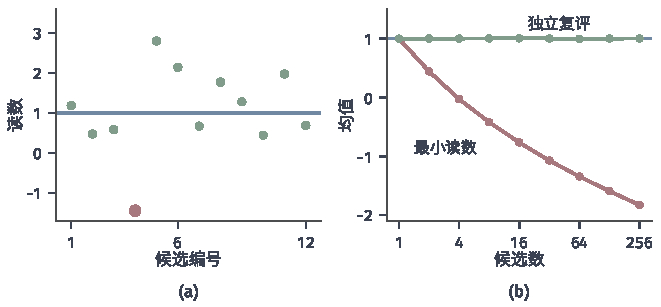
\includegraphics[width=112mm]{figures/05-optimization/05-stochastic-optimization/matplotlib/zo-selection/figure.pdf}
  \caption{含噪比较的选择偏差，真实值都是$1$（蓝线），噪声为标准正态。(a)$12$个候选的一次读数，红点是读数最低者，它并不比其他候选好。(b)红线是$K$个候选中最小读数的均值，随$K$增大而偏低；绿线是选定后独立复评的均值，始终等于真值。每点$10^5$次模拟。}
  \label{fig:zo-selection}
\end{BookInlineFigure}

\section{误差与查询成本}
\label{sec:zo-error-cost}

前面记下了各种误差的账，本节把它们合并。要解决的问题是：给定函数读数的总预算，误差由哪几部分构成，各种方法怎样比较，平滑问题上的结论又怎样回到原问题？比较时固定同一个评价预算，分开记录三种误差：平滑或差分偏差、随机方向误差和读数噪声。

\subsection{扰动尺度的取舍}
\label{sec:zo-tradeoff}

\paragraph{差商的U形曲线}
扰动太大，差商在量一段弯曲路径的平均坡度；扰动太小，一点噪声就被放大。这两股力量相反，总误差随尺度呈U形。

取均方误差分析。前向差商在二阶导有上界$L$时，偏差不超过$Lh/2$；中心差商在三阶导有上界$M$时，偏差不超过$Mh^2/6$。结合式~\eqref{eq:zo-quotient-noise}，独立噪声下的均方误差满足
\begin{equation}
 \mathrm{MSE}_{\mathrm{F}}(h)\leq\frac{L^2h^2}{4}+\frac{2\sigma^2}{h^2},\qquad
 \mathrm{MSE}_{\mathrm{C}}(h)\leq\frac{M^2h^4}{36}+\frac{\sigma^2}{2h^2}.
 \label{eq:zo-mse}
\end{equation}
第二项随$h$平方的倒数增长，这对独立的加性噪声是不可避免的。对两式右端关于$h$求导并令其为零，得到最优尺度
\begin{equation}
 h_{\mathrm{F}}=\Bigl(\frac{8\sigma^2}{L^2}\Bigr)^{1/4},\qquad
 h_{\mathrm{C}}=\Bigl(\frac{3\sigma}{M}\Bigr)^{1/3}.
 \label{eq:zo-optimal-h}
\end{equation}

继续用$\varphi(s)=s^2/2+s^3/6$，$s_0=1$，这里局部取$L=\varphi''(1)=2$，$M=1$，噪声$\sigma=0.01$。代入式~\eqref{eq:zo-optimal-h}，得到
\[
 h_{\mathrm{F}}\approx0.119,\qquad h_{\mathrm{C}}\approx0.311.
\]
最优点上的均方根误差分别约为$0.17$和$0.028$，如图~\ref{fig:zo-tradeoff}。差别不只在数值：中心差分可以用更大的$h$，这同时削弱了噪声放大，所以在噪声存在时收益比精确读数时更明显。

\begin{BookInlineFigure}
  \centering
  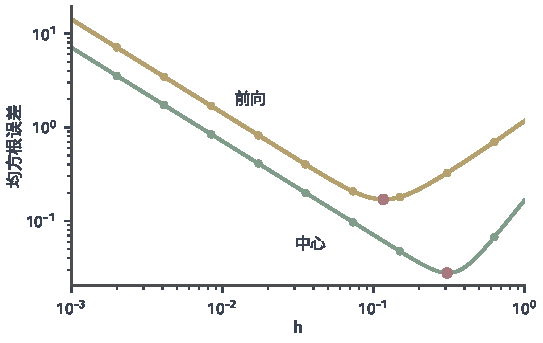
\includegraphics[width=92mm]{figures/05-optimization/05-stochastic-optimization/matplotlib/zo-tradeoff/figure.pdf}
  \caption{差商均方根误差随$h$的变化，$\varphi(s)=s^2/2+s^3/6$，$s_0=1$，独立噪声$\sigma=0.01$。黄线为前向差分，绿线为中心差分，曲线是偏差平方加方差的精确值，圆点是$2\times10^5$次模拟的结果，红点是各自的最小值。$h$小时两线斜率都是$-1$，$h$大时分别是$1$和$2$。}
  \label{fig:zo-tradeoff}
\end{BookInlineFigure}

\paragraph{迭代中的同一取舍}
在迭代算法中，平滑半径受同样的取舍支配，但记账的单位变了。定理~\ref{thm:zo-convex}的上界对$\delta$的依赖是$\alpha V+L\delta^2/2$，而$V$里的噪声项$\propto1/\delta^2$。

图~\ref{fig:zo-delta-u}用一个非二次的凸目标$f(\bm{x})=\sum_{i=1}^2(e^{x_i}-x_i-1)$做实验，解是原点，$f^\star=0$，算法跑固定轮数，噪声$\sigma=0.2$。$\delta$小的一侧，误差按$1/\delta^2$增长，来自噪声；$\delta$大的一侧，平滑目标的解偏离原点，误差快速上升。最好的$\delta$在$0.5$附近，目标差约$0.0026$，$\delta=0.02$和$\delta=4$时都超过$1$。

\begin{BookInlineFigure}
  \centering
  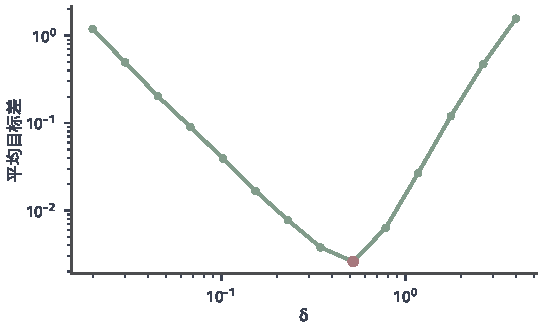
\includegraphics[width=92mm]{figures/05-optimization/05-stochastic-optimization/matplotlib/zo-delta-u/figure.pdf}
  \caption{双点方法在$f(\bm{x})=\sum_{i=1}^2(e^{x_i}-x_i-1)$上的平均目标差随$\delta$的变化，起点$(1,1)$，$\alpha=0.02$，$\sigma=0.2$，$T=3000$，取最后$500$步的平均，$200$次运行。左支由噪声放大主导，右支由平滑偏差主导，红点是扫描到的最小值。}
  \label{fig:zo-delta-u}
\end{BookInlineFigure}

\paragraph{共享样本时规律不同}
上面的$1/\delta^2$规律只适用于独立加性噪声。共享的Lipschitz样本下，差商的方差不随$\delta$增大而爆炸，$\delta$可以尽量取小，U形曲线的左支几乎消失。而指示函数样本的方差$\propto1/\delta$，左支依然存在，只是坡度减半。用哪个$\delta$要先确定噪声模型。

\subsection{维数与方向数}
\label{sec:zo-dimension}

“每轮只读两次”常被误解成成本与维数无关。上面的$\alpha\lesssim1/(nL)$已经说明，维数并没有消失，只是从每轮的读数次数转移到了步长上。

\paragraph{单轮比较}
表~\ref{tab:zo-moments}比较完整坐标差分和随机方向在单轮的成本与误差。这里的“方向波动”是读数精确时二次函数上的$\mathbb{E}\lVert\hat{\bm{g}}-\bm{g}\rVert_2^2$。

\begin{BookInlineTable}
  \centering
  \begin{tabular}{@{}llll@{}}
    \toprule
    方法 & 单轮读数 & 方向波动 & 独立噪声贡献\\
    \midrule
    中心坐标 & $2n$ & $0$ & $n\sigma^2/(2h^2)$\\
    单方向对称 & $2$ & $(n-1)\lVert\bm{g}\rVert_2^2$ & $n^2\sigma^2/(2\delta^2)$\\
    $m$方向对称 & $2m$ & $(n-1)\lVert\bm{g}\rVert_2^2/m$ & $n^2\sigma^2/(2m\delta^2)$\\
    $m$方向共用中心 & $m+1$ & 取决于函数 & $2n^2\sigma^2/(m\delta^2)$\\
    \bottomrule
  \end{tabular}
  \caption{一轮估计的成本与误差。$m=n$时，随机方向的噪声贡献与中心坐标差分相同，都是$n\sigma^2/(2\delta^2)$，读数次数也相同。}
  \label{tab:zo-moments}
\end{BookInlineTable}

\paragraph{相同预算下的结果}
图~\ref{fig:zo-dims}在$n=20$的二次目标上比较三种配置，步长按单轮二阶矩调节：坐标差分用$1/L$，$m$方向平均用$1/(L(1+(n-1)/m))$。横轴都是函数读数次数。读数精确时三条线基本平行，图(a)；读数含噪时停在几乎同一水平，图(b)。

\begin{BookInlineFigure}
  \centering
  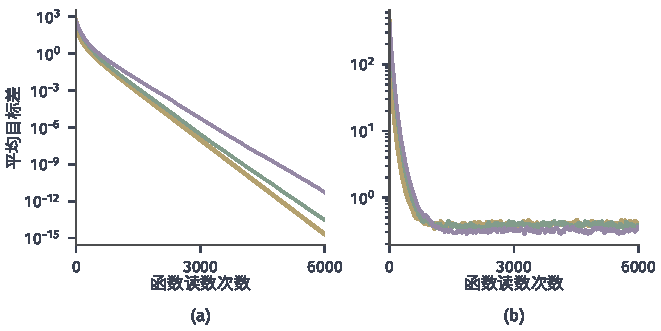
\includegraphics[width=112mm]{figures/05-optimization/05-stochastic-optimization/matplotlib/zo-dims/figure.pdf}
  \caption{$n=20$的二次目标，$\bm{H}$的对角元从$1$均匀到$9$，$h=\delta=0.1$，$30$次运行平均。黄线：中心坐标差分。绿线：$m=1$的随机方向。紫线：$m=5$的随机方向。(a)读数精确。(b)独立噪声$\sigma=0.1$。按读数次数计，三者的差别远小于“两次查询对$40$次查询”的字面差距。}
  \label{fig:zo-dims}
\end{BookInlineFigure}

这个实验的结论有范围。它说明在按读数计费、读数可独立提交的情形下，每轮少读并不等于总成本少。随机方向的优势在别处：可以在读完所有坐标之前就开始移动。梯度集中在少数方向时效果可能更好，但这取决于具体结构，本章没有相应的定理。反过来，如果读数可并行、每轮墙钟时间固定，完整差分反而可能更快。

\paragraph{方向平均与共用中心读数}
独立方向平均把方差除以$m$，这部分依赖独立性。为节省读数，有人让所有方向共用一次中心读数$y_0=f(\bm{x})+\zeta_0$，读数次数从$2m$降到$m+1$。这时
\[
 \hat{\bm{g}}=\frac{n}{\delta m}\sum_{j=1}^m(y_j-y_0)\bm{u}_j,
\]
噪声部分是$\tfrac{n}{\delta m}\sum_j(\zeta_j-\zeta_0)\bm{u}_j$。给定方向，$\zeta_0$对所有方向是同一个数，噪声不再独立，二阶矩是
\[
 \frac{n^2\sigma^2}{\delta^2m^2}\Bigl(m+\Bigl\lVert\sum_{j=1}^m\bm{u}_j\Bigr\rVert_2^2\Bigr).
\]
方向独立随机时$\mathbb{E}\lVert\sum_j\bm{u}_j\rVert_2^2=m$，总贡献是$2n^2\sigma^2/(m\delta^2)$，与每方向单独读中心点的情形相同。方向相关时，比如都偏向同一侧，第二项可以高达$m^2$。所以共用中心读数引入了相关性，必须单独计入。

坐标方向上这一点最清楚。前向坐标差分共用$f(\bm{x})$时，噪声的协方差是
\[
 \frac{\sigma^2}{h^2}\bigl(\bm{I}+\bm{1}\bm{1}^\top\bigr),
\]
它的特征值是$(n+1)\sigma^2/h^2$（对应方向$\bm{1}$）和$n-1$个$\sigma^2/h^2$。公共噪声把误差压到一个方向上，如图~\ref{fig:zo-cov}(a)，而中心差分的误差是各向同性的，如图(b)。

\begin{BookInlineFigure}
  \centering
  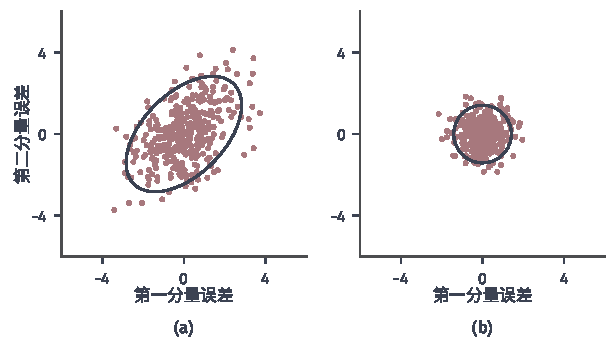
\includegraphics[width=104mm]{figures/05-optimization/05-stochastic-optimization/matplotlib/zo-cov/figure.pdf}
  \caption{$n=2$，$\sigma=h=0.1$时坐标差分的噪声误差。红点是$350$次模拟，黑色椭圆是两倍标准差的等概率线。(a)前向差分共用中心读数，协方差$\begin{bmatrix}2&1\\1&2\end{bmatrix}$，误差沿$(1,1)$方向拉长。(b)中心差分，协方差为$\tfrac12\bm{I}$。}
  \label{fig:zo-cov}
\end{BookInlineFigure}

\subsection{原目标的误差评价}
\label{sec:zo-original-error}

第~\ref{sec:zo-output}节的定理说的都是平滑目标。原来要解决的问题是最小化$f$，本小节补上这一步。

\paragraph{函数平滑误差}
设平滑目标$f_{\mathrm{s}}$与$f$处处至多相差$\gamma_f$，这个常数$\gamma_f$是\term{函数平滑误差}（function smoothing error）。由引理~\ref{lem:zo-smoothing-properties}，光滑函数的球平滑可取$\gamma_f=L\delta^2/2$，$G$-Lipschitz函数可取$\gamma_f=G\delta$。

\begin{theorem}[从平滑目标回到原目标]
\label{thm:zo-transfer}
设$\lvert f_{\mathrm{s}}-f\rvert\leq\gamma_f$，$\bm{x}^\star$是$f$的解，则对任意$\hat{\bm{x}}$，
\begin{equation}
 f(\hat{\bm{x}})-f^\star\leq f_{\mathrm{s}}(\hat{\bm{x}})-f_{\mathrm{s}}(\bm{x}^\star)+2\gamma_f.
 \label{eq:zo-function-transfer}
\end{equation}
若两者的梯度处处至多相差$\gamma_g$（按欧氏范数），则
\begin{equation}
 \lVert\nabla f(\hat{\bm{x}})\rVert_2^2\leq2\lVert\nabla f_{\mathrm{s}}(\hat{\bm{x}})\rVert_2^2+2\gamma_g^2.
 \label{eq:zo-gradient-transfer}
\end{equation}
\end{theorem}

\begin{proof}
由一致误差的假设，
\[
 f(\hat{\bm{x}})\leq f_{\mathrm{s}}(\hat{\bm{x}})+\gamma_f,\qquad f_{\mathrm{s}}(\bm{x}^\star)\leq f^\star+\gamma_f.
\]
两式相加移项得式~\eqref{eq:zo-function-transfer}。

由三角不等式，$\lVert\nabla f\rVert_2$不超过$\lVert\nabla f_{\mathrm{s}}\rVert_2+\gamma_g$，两边平方并用$(a+b)^2\leq2a^2+2b^2$，得式~\eqref{eq:zo-gradient-transfer}。
\end{proof}

式~\eqref{eq:zo-function-transfer}中的$2\gamma_f$在凸函数上可以省一半，因为$f\leq f^{\mathrm{B}}_{\delta}$。把定理~\ref{thm:zo-convex}代回，对光滑凸目标得到
\begin{equation}
 \mathbb{E}f(\bar{\bm{x}})-f^\star\leq\frac{R_0^2}{\alpha T}+\alpha V+L\delta^2.
 \label{eq:zo-convex-original}
\end{equation}
把定理~\ref{thm:zo-nonconvex}代回，取$\gamma_g=L\delta$，对光滑非凸目标得到
\begin{equation}
 \mathbb{E}\bigl\lVert\nabla f(\bm{x}^{(R)})\bigr\rVert_2^2\leq\frac{4\Delta_\delta}{\alpha T}+2L\alpha W+2L^2\delta^2.
 \label{eq:zo-nonconvex-original}
\end{equation}

\paragraph{平滑目标的解不是原目标的解}
这个换算的$\gamma_f$是不能省的。取$f(x)=\max\{x,-2x\}$，$n=1$，$\delta=1$，解是$x^\star=0$。$\lvert x\rvert<1$时，平滑目标的导数是
\[
 \bigl(f^{\mathrm{B}}_{\delta}\bigr)'(x)=\frac{f(x+1)-f(x-1)}{2}=\frac{3x-1}{2},
\]
零点在$x=1/3$，如图~\ref{fig:zo-asym}(a)。平滑目标的精确解带着原目标差$f(1/3)=1/3$。原目标两侧的斜率不对称，平均之后最低点向缓的一侧移动。这笔误差不是算法或噪声造成的，平滑的定义本身就带来了它。

\begin{BookInlineFigure}
  \centering
  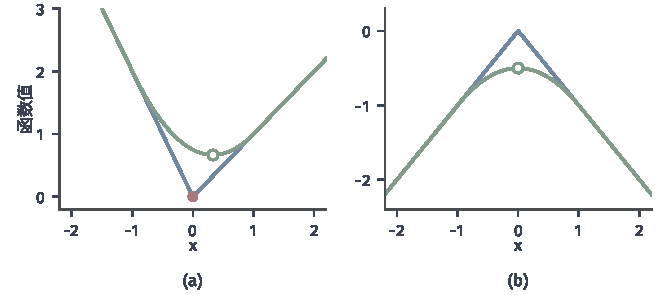
\includegraphics[width=112mm]{figures/05-optimization/05-stochastic-optimization/matplotlib/zo-asym/figure.pdf}
  \caption{平滑目标（绿）与原目标（蓝）的差别，$\delta=1$，一维区间平均。(a)$f(x)=\max\{x,-2x\}$，原解是红点$x=0$，平滑目标的解是空心点$x=1/3$，不在原解上。(b)$f(x)=-\lvert x\rvert$，平滑后在$x=0$处导数为零（空心点），而$x=0$是原函数的极大点。}
  \label{fig:zo-asym}
\end{BookInlineFigure}

\paragraph{原目标不光滑时要换驻点的概念}
式~\eqref{eq:zo-gradient-transfer}需要$\nabla f$存在且$\gamma_g$有限。原目标不可微时，平滑梯度小不能说明原目标梯度小。回到$f=\lvert x\rvert$，由$\bigl(f^{\mathrm{B}}_{\delta}\bigr)'(x)=x/\delta$，在$x=0.01\delta$处平滑导数只有$0.01$，而原函数在此处的导数是$1$。

平滑梯度小给出的是另一种结论。$f$是Lipschitz时，$\nabla f^{\mathrm{B}}_{\delta}(\bm{x})$是$\delta$邻域内各点梯度的平均，所以它小，说明邻域内的梯度有一个小的平均。这是Goldstein意义下的$\delta$驻点，比经典驻点弱。

这也不保证全局最优。图~\ref{fig:zo-asym}(b)的$f=-\lvert x\rvert$，平滑后$x=0$处导数为零，而$x=0$恰恰是原函数的极大点。更一般的多谷目标上，平滑可能磨掉一些浅谷，但没有定理保证平滑目标的驻点在全局最优点附近。

\subsection{函数评估总成本}
\label{sec:zo-total-cost}

\paragraph{成本的组成}
一次优化消耗的函数读数总数是
\begin{equation}
 Q=T\cdot m\cdot q\cdot r+Q_{\mathrm{eval}},
 \label{eq:zo-total-cost}
\end{equation}
其中$T$是迭代轮数，$m$是每轮方向数，$q$是每方向的查询次数，$r$是每个查询点的重复测量次数，$Q_{\mathrm{eval}}$是最终复评的开销。

取$T=200$，$m=2$，$q=2$，$r=3$，末了对$5$个候选各复评$20$次，代入式~\eqref{eq:zo-total-cost}，得到
\[
 Q=200\cdot2\cdot2\cdot3+5\cdot20=2500.
\]
重复测量$r$和扰动尺度$\delta$都能减小差商的噪声，但是方式不同：$r$把方差除以$r$，代价是读数翻$r$倍；增大$\delta$不需要额外读数，但引入偏差。

\paragraph{并行耗时与评估总量}
总量$Q$和实际等待时间是两个量。如果有$12$个并行的仿真槽，上例每轮的$12$次读数可同时提交，迭代部分需要$200$个批次，复评$100$次需要$9$个批次，总共$209$批。单线运行时就是$2500$次。比较算法时要说明用的是哪一个。并行时完整差分的劣势大大减小，甚至可能占优，因为它的每一轮都同时做完。

\paragraph{达到指定精度的成本}
下面把前面的上界解出来，得到达到精度$\varepsilon$所需的读数量级。$\sigma$是独立噪声的标准差。

读数精确且$f$是$L$-光滑凸函数时，由式~\eqref{eq:zo-convex-original}，$V=n^2L^2\delta^2/2$。取$\alpha=1/(4nL)$，上界是
\[
 \frac{4nLR_0^2}{T}+\Bigl(\frac{n}{8}+1\Bigr)L\delta^2.
\]
$\delta$可以任意小，只受浮点精度的限制。取$\delta^2\leq\varepsilon/((2+n/4)L)$，$T=8nLR_0^2/\varepsilon$，每轮两次读数，得到
\[
 Q=\frac{16\,nLR_0^2}{\varepsilon}.
\]
梯度下降需要$O(LR_0^2/\varepsilon)$次梯度，这里多出的正是因子$n$，同完整坐标差分的成本同阶。

独立噪声下，由式~\eqref{eq:zo-convex-original}和$V\approx n^2\sigma^2/(2\delta^2)$，把步长调到最优后上界约为
\[
 2R_0\sqrt{\frac{V}{T}}+L\delta^2=\frac{\sqrt{2}R_0n\sigma}{\delta\sqrt{T}}+L\delta^2.
\]
对$\delta$求最小，得$\delta\propto T^{-1/6}$，误差$\varepsilon\propto T^{-1/3}$，反解$T$得到$Q=O(LR_0^2n^2\sigma^2/\varepsilon^3)$。这里$\delta$必须随预算一起缩小，否则$L\delta^2$这项不消失。这是第~\ref{sec:zo-tradeoff}节U形曲线在迭代算法中的结果。

只有单点反馈且$f$是$G$-Lipschitz凸函数、$\lvert f\rvert\leq B$时，二阶矩是$n^2B^2/\delta^2$，平滑误差是$G\delta$。同样的累加分析给出误差约$R_0nB/(\delta\sqrt{T})+G\delta$，最优化$\delta$后$\varepsilon\propto T^{-1/4}$。

光滑非凸情形按式~\eqref{eq:zo-nonconvex-original}同样处理。精确读数时取足够小的$\delta$，$\alpha=1/(4nL)$，得$Q=O(nL\Delta/\varepsilon^2)$，这里$\Delta$是初始目标与下界之差。独立噪声时平衡$\delta$，得$\varepsilon^2\propto T^{-1/3}$，反解得表中的量级。

表~\ref{tab:zo-costs}汇总这些结果。

\begin{BookInlineTable}
  \centering
  \begin{tabular}{@{}lll@{}}
    \toprule
    反馈与正则性 & 估计器 & 读数量级\\
    \midrule
    精确，$L$-光滑凸 & 双点球面 & $nLR_0^2/\varepsilon$\\
    精确，$L$-光滑非凸 & 双点球面 & $nL\Delta/\varepsilon^2$\\
    独立噪声，$L$-光滑凸 & 双点球面 & $LR_0^2n^2\sigma^2/\varepsilon^3$\\
    独立噪声，$L$-光滑非凸 & 双点球面 & $L^3\Delta n^2\sigma^2/\varepsilon^6$\\
    单点，$G$-Lipschitz凸，$\lvert f\rvert\leq B$ & 单点球面 & $n^2R_0^2B^2G^2/\varepsilon^4$\\
    共享Lipschitz样本，凸 & 双点球面 & $n^2G^2R_0^2/\varepsilon^2$\\
    \bottomrule
  \end{tabular}
  \caption{本章简单估计器达到精度$\varepsilon$的读数量级，略去常数。凸问题的精度指目标差，非凸问题指$\lVert\nabla f\rVert_2\leq\varepsilon$；末行由$\lVert\hat{\bm{g}}\rVert_2\leq nG$的粗略界得到。这些都是上界，不是问题本身的下界。}
  \label{tab:zo-costs}
\end{BookInlineTable}

表的最后一行可以改进。利用球面上Lipschitz函数的集中不等式，双点估计的二阶矩能够改进到$O(nG^2)$，读数量级相应地变成$nG^2R_0^2/\varepsilon^2$。这一步的证明需要用到球面集中不等式，篇幅较长，读者可查阅Duchi等人及Shamir关于双点反馈的工作。它的含义是：共享样本下，配对的收益是把维数从平方降到一次方。

比较时要留意三件事。一是接口：表中的噪声列不能跨行混用，独立噪声的速率不适用于共享样本，反之亦然。二是度量：目标差和梯度范数的$\varepsilon$不是一回事。三是假设：更好的指数往往需要更强的光滑性和更复杂的估计器，不是换一个步长就能得到。

\section{本章小结}
\label{sec:zo-summary}

本章在只能读函数值的条件下回答了怎样构造方向、怎样迭代、最后得到什么保证。函数值反馈先要说清接口：精确值、加性噪声和样本函数是三种读数模型，单点与成对、独立噪声与共享样本是不同的读取条件，算法抽方向的随机性与读数的随机性分开记录。

局部方向有两种读法。有限差分以原梯度为对象：坐标差分需要$n+1$或$2n$次读数，随机方向差分和SPSA只需两次，但一条方向只有一条方向的信息，有限扰动下一般有偏，SPSA的坐标尺度乘以$\sqrt{n}$才是位移长度。随机平滑以平滑目标为对象：球平滑的恒等式~\eqref{eq:zo-ball-identity}和高斯平滑的恒等式~\eqref{eq:zo-gauss-identity}给出严格无偏的估计，单点估计受函数值大小影响，双点估计消去常数偏移。独立噪声让差商方差按$1/\delta^2$增长，共享样本是否改善取决于差值的波动。

把估计器代入迭代后，算法实际优化的目标由条件均值决定。步长受维数限制约为$1/(nL)$，扰动尺度决定平滑目标和噪声，缩小它要同时记入目标变化和方差增长。约束下要分清更新可行与查询可行，球形扰动可用收缩集合，高斯扰动有无界支撑。输出按问题选择平均点或随机返回点，预算耗尽、读数不变和驻点保证是不同的停止依据，含噪比较需要独立复评。

按读数计费时，两次查询并不代表成本与维数无关，因子$n$转移到了步长上。平滑目标上的结论要加上平滑误差才是原目标的结论，原目标不光滑时平滑梯度小只是较弱的驻点概念，也不保证全局最优。选择方法时，先看接口：能读坐标且读数便宜就用差分；扰动必须同时施加时用SPSA；只有单点反馈时用单点估计；能共享样本时优先双点估计并尽量取小$\delta$。

高斯平滑的恒等式也可以看作：把$\bm{x}$当作高斯搜索分布的均值，这个估计描述均值移动时平均目标的变化。第~\ref{chap:random-search}章继续讨论怎样更新搜索分布和种群，那里的方法不都等同于本章的零阶梯度下降。

